\section{寄存器描述}
\regover{
{\hyperref[SDH-SDMA-System-Address-Argument-2]{SDMA\_System\_Address\_Argument\_2}}&
\\
\hline
{\hyperref[SDH-Block-Size]{Block\_Size}}&
\\
\hline
{\hyperref[SDH-Block-Count]{Block\_Count}}&
\\
\hline
{\hyperref[SDH-Argument-1]{Argument\_1}}&
\\
\hline
{\hyperref[SDH-Transfer-Mode]{Transfer\_Mode}}&
\\
\hline
{\hyperref[SDH-Command]{Command}}&
\\
\hline
{\hyperref[SDH-Response-1]{Response\_1}}&
\\
\hline
{\hyperref[SDH-Response-2]{Response\_2}}&
\\
\hline
{\hyperref[SDH-Response-3]{Response\_3}}&
\\
\hline
{\hyperref[SDH-Response-4]{Response\_4}}&
\\
\hline
{\hyperref[SDH-Buffer-Data-Port]{Buffer\_Data\_Port}}&
\\
\hline
{\hyperref[SDH-Present-State]{Present\_State}}&
\\
\hline
{\hyperref[SDH-Host-Control-1]{Host\_Control\_1}}&
\\
\hline
{\hyperref[SDH-Power-Control]{Power\_Control}}&
\\
\hline
{\hyperref[SDH-Block-Gap-Control]{Block\_Gap\_Control}}&
\\
\hline
{\hyperref[SDH-Wakeup-Control]{Wakeup\_Control}}&
\\
\hline
{\hyperref[SDH-Clock-Control]{Clock\_Control}}&
\\
\hline
{\hyperref[SDH-Timeout-Control]{Timeout\_Control}}&
\\
\hline
{\hyperref[SDH-Software-Reset]{Software\_Reset}}&
\\
\hline
{\hyperref[SDH-Normal-Interrupt-Status]{Normal\_Interrupt\_Status}}&
\\
\hline
{\hyperref[SDH-Error-Interrupt-Status]{Error\_Interrupt\_Status}}&
\\
\hline
{\hyperref[SDH-Normal-Interrupt-Status-Enable]{Normal\_Interrupt\_Status\_Enable}}&
\\
\hline
{\hyperref[SDH-Error-Interrupt-Status-Enable]{Error\_Interrupt\_Status\_Enable}}&
\\
\hline
{\hyperref[SDH-Normal-Interrupt-Signal-Enable]{Normal\_Interrupt\_Signal\_Enable}}&
\\
\hline
{\hyperref[SDH-Error-Interrupt-Signal-Enable]{Error\_Interrupt\_Signal\_Enable}}&
\\
\hline
{\hyperref[SDH-Auto-CMD-Error-Status]{Auto\_CMD\_Error\_Status}}&
\\
\hline
{\hyperref[SDH-Host-Control-2]{Host\_Control\_2}}&
\\
\hline
{\hyperref[SDH-Capabilities-1]{Capabilities\_1}}&
\\
\hline
{\hyperref[SDH-Capabilities-2]{Capabilities\_2}}&
\\
\hline
{\hyperref[SDH-Maximum-Current-Capabilities]{Maximum\_Current\_Capabilities}}&
\\
\hline
{\hyperref[SDH-Force-Event-Register-for-Auto-CMD-Error-Status]{Force\_Event\_Register\_for\_Auto\_CMD\_Error\_Status}}&
\\
\hline
{\hyperref[SDH-Force-Event-Register-for-Error-Interrupt-Status]{Force\_Event\_Register\_for\_Error\_Interrupt\_Status}}&
\\
\hline
{\hyperref[SDH-ADMA-Error-Status]{ADMA\_Error\_Status}}&
\\
\hline
{\hyperref[SDH-Shared-Bus-Control]{Shared\_Bus\_Control}}&
\\
\hline
{\hyperref[SDH-Slot-Interrupt-Status]{Slot\_Interrupt\_Status}}&
\\
\hline
{\hyperref[SDH-Host-Controller-Version]{Host\_Controller\_Version}}&
\\
\hline
}

\subsection{SDMA\_System\_Address\_Argument\_2}
\label{SDH-SDMA-System-Address-Argument-2}
地址:0x20060000
 \begin{figure}[H]
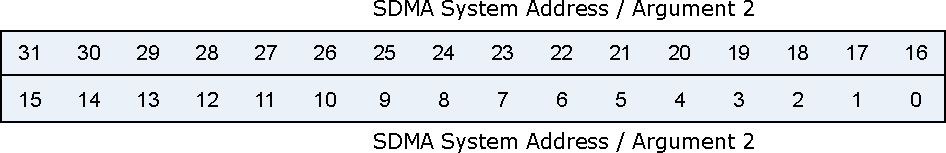
\includegraphics{SDH_SDMA_System_Address_Argument_2.pdf}
\end{figure}

\regdes{31:0&SDMASystem&r/w&32'd0&SDMA System Address / Argument 2  \par This register contains the physical system memory address used for DMA transfers  \par or the second argument for the Auto CMD23.  \par (1) SDMA System Address \par This register contains the system memory address for a SDMA transfer. When  \par the Host Controller stops a SDMA transfer, this register shall point to the system  \par address of the next contiguous data position. It can be accessed only if no  \par transaction is executing (i.e., after a transaction has stopped). Read operations  \par during transfers may return an invalid value.  \par (2) Argument 2 \par This register is used with the Auto CMD23 to set a 32-bit block count value to  \par the argument of the CMD23 while executing Auto CMD23. 
\\\hline

}
\subsection{Block\_Size}
\label{SDH-Block-Size}
地址:0x20060004
 \begin{figure}[H]
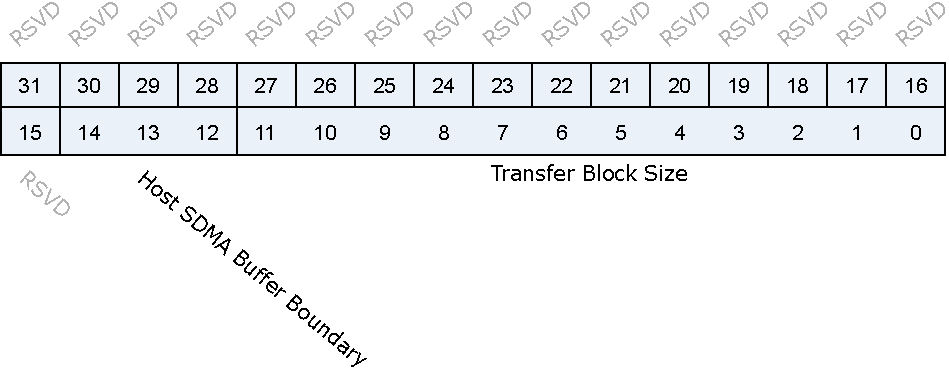
\includegraphics{SDH_Block_Size.pdf}
\end{figure}

\regdes{31:15&RSVD& & & \\\hline
14:12&HostSDMA&r/w&3'd0&Host SDMA Buffer Boundary  \par The large contiguous memory space may not be available in the virtual memory  \par system. To perform long SDMA transfer, SDMA System Address register shall be  \par updated at every system memory boundary during SDMA transfer.  \par These bits specify the size of contiguous buffer in the system memory. The  \par SDMA transfer shall wait at the every boundary specified by these fields and the  \par Host Controller generates the DMA Interrupt to request the Host Driver to  \par update the SDMA System Address register. At the end of transfer, the Host  \par Controller may issue or may not issue DMA Interrupt. In particular, DMA  \par Interrupt shall not be issued after Transfer Complete Interrupt is issued.  \par In case of this register is set to 0 (buffer size = 4K bytes), lower 12-bit of byte  \par address points data in the contiguous buffer and the upper 20-bit points the  \par location of the buffer in the system memory. The SDMA transfer stops when the  \par Host Controller detects carry out of the address from bit 11 to 12.  \par These bits shall be supported when the SDMA Support in the Capabilities \par register is set to 1 and this function is active when the DMA Enable in the  \par Transfer Mode register is set to 1. ADMA does not use this register.
\\\hline
11:0&TransferBlock&r/w&12'b0&Transfer Block Size  \par This register specifies the block size of data transfers for CMD17, CMD18,  \par CMD24, CMD25, and CMD53. Values ranging from 1 up to the maximum buffer  \par size can be set. In case of memory, it shall be set up to 512 bytes (Refer to  \par Implementation Note in Section 1.7.2). It can be accessed only if no transaction  \par is executing (i.e., after a transaction has stopped). Read operations during  \par transfers may return an invalid value, and write operations shall be ignored. 
\\\hline

}
\subsection{Block\_Count}
\label{SDH-Block-Count}
地址:0x20060006
 \begin{figure}[H]
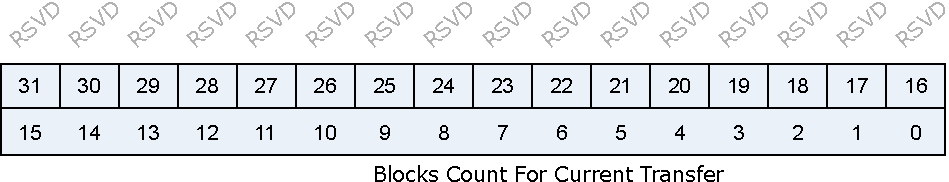
\includegraphics{SDH_Block_Count.pdf}
\end{figure}

\regdes{31:16&RSVD& & & \\\hline
15:0&BlocksCount&r/w&16'd0&Blocks Count For Current Transfer  \par This register is enabled when Block Count Enable in the Transfer Mode register is  \par set to 1 and is valid only for multiple block transfers. The Host Driver shall set this  \par register to a value between 1 and the maximum block count. The Host Controller  \par decrements the block count after each block transfer and stops when the count  \par reaches zero. Setting the block count to 0 results in no data blocks is transferred.  \par This register should be accessed only when no transaction is executing (i.e., after  \par transactions are stopped). During data transfer, read operations on this register may  \par return an invalid value and write operations are ignored.  \par When a suspend command is completed, the number of blocks yet to be transferred  \par can be determined by reading this register. Before issuing a resume command, the  \par Host Driver shall restore the previously saved block count. 
\\\hline

}
\subsection{Argument\_1}
\label{SDH-Argument-1}
地址:0x20060008
 \begin{figure}[H]
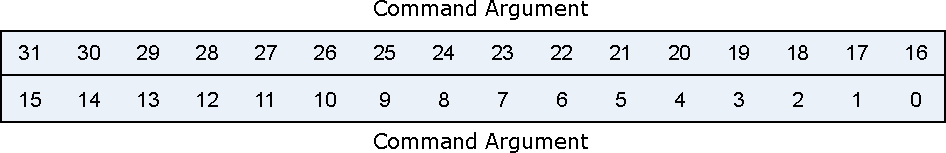
\includegraphics{SDH_Argument_1.pdf}
\end{figure}

\regdes{31:0&CommandArgument&r/w&32'h0&Command Argument 1  \par The SD command argument is specified as bit39-8 of Command-Format in the  \par Physical Layer Specification.
\\\hline

}
\subsection{Transfer\_Mode}
\label{SDH-Transfer-Mode}
地址:0x2006000c
 \begin{figure}[H]
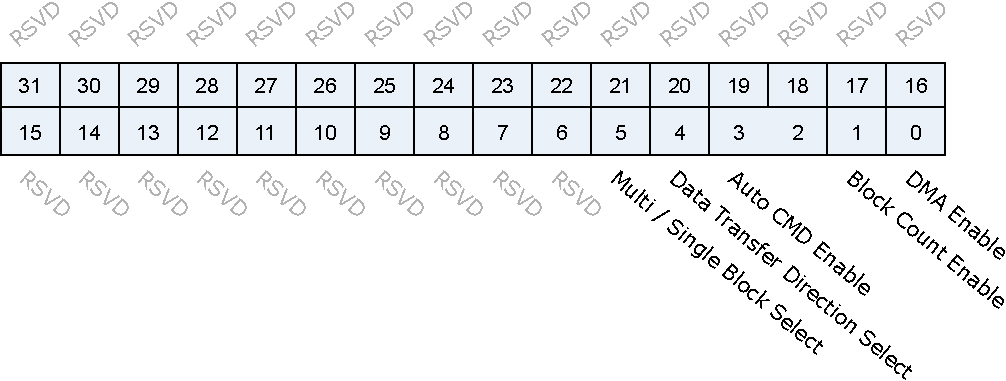
\includegraphics{SDH_Transfer_Mode.pdf}
\end{figure}

\regdes{31:6&RSVD& & & \\\hline
5&Multi/&r/w&1'b0&Multi / Single Block Select  \par This bit is set when issuing multiple-block transfer commands using DAT line. For  \par any other commands, this bit shall be set to 0. If this bit is 0, it is not necessary to  \par set the Block Count register. (Refer to Table 2-8) 
\\\hline
4&DataTransfer&r/w&1'b0&Data Transfer Direction Select  \par This bit defines the direction of DAT line data transfers. The bit is set to 1 by the  \par Host Driver to transfer data from the SD card to the SD Host Controller and it is  \par set to 0 for all other commands. 
\\\hline
3:2&AutoCMD&r/w&2'd0&Auto CMD Enable  \par This field determines use of auto command functions.  \par (1) Auto CMD12 Enable  \par (2) Auto CMD23 Enable 
\\\hline
1&BlockCount&r/w&1'b0&This bit is used to enable the Block Count register, which is only relevant for  \par multiple block transfers. When this bit is 0, the Block Count register is disabled,  \par which is useful in executing an infinite transfer. \par If ADMA2 data transfer is more than 65535 blocks, this bit shall be set to 0. In this  \par case, data transfer length is designated by Descriptor Table. 
\\\hline
0&DMAEnable&r/w&1'b0&This bit enables DMA functionality as described in section 1.4. DMA can be  \par enabled only if it is supported as indicated in the Capabilities register. One of the  \par DMA modes can be selected by DMA Select in the Host Control 1 register. If  \par DMA is not supported, this bit is meaningless and shall always read 0. If this bit is  \par set to 1, a DMA operation shall begin when the Host Driver writes to the upper  \par byte of Command register (00Fh).
\\\hline

}
\subsection{Command}
\label{SDH-Command}
地址:0x2006000e
 \begin{figure}[H]
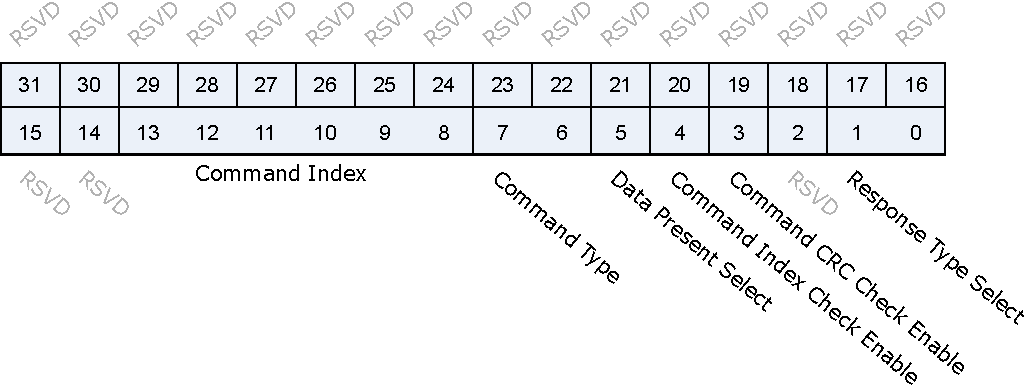
\includegraphics{SDH_Command.pdf}
\end{figure}

\regdes{31:14&RSVD& & & \\\hline
13:8&CommandIndex&r/w&6'd0&These bits shall be set to the command number (CMD0-63, ACMD0-63) that is  \par specified in bits 45-40 of the Command-Format in the Physical Layer  \par Specification and SDIO Card Specification.
\\\hline
7:6&CommandType&r/w&2'd0&There are three types of special commands: Suspend, Resume and Abort.  \par These bits shall be set to 00b for all other commands.  \par (1) Suspend Command  \par (2) Resume Command  \par (3) Abort Command  
\\\hline
5&DataPresent&r/w&1'b0&This bit is set to 1 to indicate that data is present and shall be transferred using  \par the DAT line. It is set to 0 for the following:  \par (1) Commands using only CMD line (ex. CMD52).  \par (2) Commands with no data transfer but using busy signal on DAT[0] line  \par (R1b or R5b ex. CMD38)  \par (3) Resume command 
\\\hline
4&CommandIndex&r/w&1'b0&If this bit is set to 1, the Host Controller shall check the Index field in the  \par response to see if it has the same value as the command index. If it is not, it is  \par reported as a Command Index Error. If this bit is set to 0, the Index field is not  \par checked. 
\\\hline
3&CommandCRC&r/w&1'b0&If this bit is set to 1, the Host Controller shall check the CRC field in the  \par response. If an error is detected, it is reported as a Command CRC Error. If this  \par bit is set to 0, the CRC field is not checked. The position of CRC field is  \par determined according to the length of the response. (Refer to definition in  \par D01-00 and Table 2-10 below.) 
\\\hline
2&RSVD& & & \\\hline
1:0&ResponseType&r/w&2'd0&00: No Response  \par 01: Response Length 136  \par 10: Response Length 48  \par 11: Response Length 48 check Busy after response
\\\hline

}
\subsection{Response\_1}
\label{SDH-Response-1}
地址:0x20060010
 \begin{figure}[H]
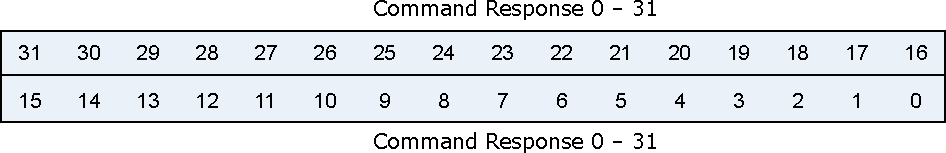
\includegraphics{SDH_Response_1.pdf}
\end{figure}

\regdes{31:0&CommandResponse&r/w&32'h0&Command Response \\\hline

}
\subsection{Response\_2}
\label{SDH-Response-2}
地址:0x20060014
 \begin{figure}[H]
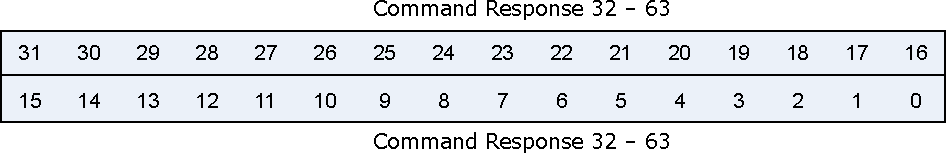
\includegraphics{SDH_Response_2.pdf}
\end{figure}

\regdes{31:0&CommandResponse&r/w&32'h0&Command Response \\\hline

}
\subsection{Response\_3}
\label{SDH-Response-3}
地址:0x20060018
 \begin{figure}[H]
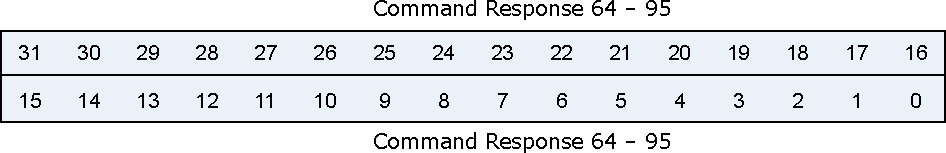
\includegraphics{SDH_Response_3.pdf}
\end{figure}

\regdes{31:0&CommandResponse&r/w&32'h0&Command Response \\\hline

}
\subsection{Response\_4}
\label{SDH-Response-4}
地址:0x2006001c
 \begin{figure}[H]
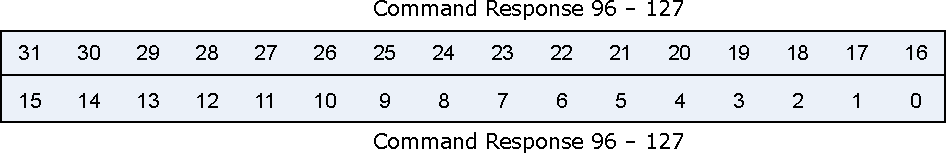
\includegraphics{SDH_Response_4.pdf}
\end{figure}

\regdes{31:0&CommandResponse&r/w&32'h0&Command Response \\\hline

}
\subsection{Buffer\_Data\_Port}
\label{SDH-Buffer-Data-Port}
地址:0x20060020
 \begin{figure}[H]
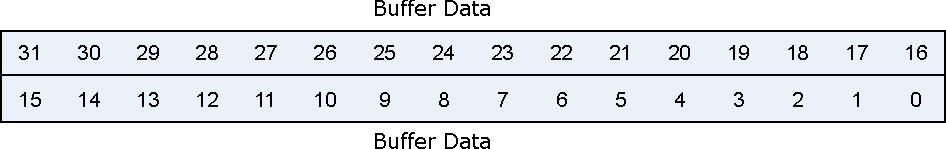
\includegraphics{SDH_Buffer_Data_Port.pdf}
\end{figure}

\regdes{31:0&BufferData&r/w&32'h0&Buffer Data  \par The Host Controller buffer can be accessed through this 32-bit Data Port register. 
\\\hline

}
\subsection{Present\_State}
\label{SDH-Present-State}
地址:0x20060024
 \begin{figure}[H]
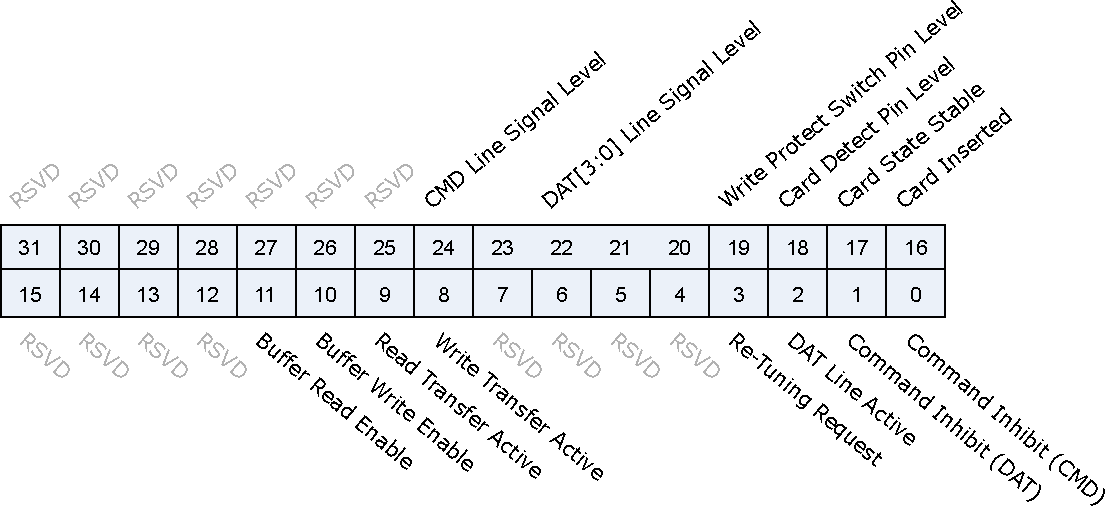
\includegraphics{SDH_Present_State.pdf}
\end{figure}

\regdes{31:25&RSVD& & & \\\hline
24&CMDLine&r&1'b0&CMD Line Signal Level  \par This status is used to check the CMD line level to recover from errors, and  \par for debugging. 
\\\hline
23:20&DAT[3:0]Line&r&4'd0&DAT[3:0] Line Signal Level  \par This status is used to check the DAT line level to recover from errors, and for  \par debugging. This is especially useful in detecting the busy signal level from  \par DAT[0]. 
\\\hline
19&WriteProtect&r&1'b0&The Write Protect Switch is supported for memory and combo cards.  \par This bit reflects the SDWP\# pin. 
\\\hline
18&CardDetect&r&1'b0&This bit reflects the inverse value of the SDCD\# pin. Debouncing is not  \par performed on this bit. This bit may be valid when Card State Stable is set to  \par 1, but it is not guaranteed because of propagation delay. Use of this bit is  \par limited to testing since it must be debounced by software. 
\\\hline
17&CardState&r&1'b0&This bit is used for testing. If it is 0, the Card Detect Pin Level is not stable.  \par If this bit is set to 1, it means the Card Detect Pin Level is stable. No Card  \par state can be detected by this bit is set to 1 and Card Inserted is set to 0. The  \par Software Reset For All in the Software Reset register shall not affect this  \par bit. 
\\\hline
16&CardInserted&r&1'b0&This bit indicates whether a card has been inserted. The Host Controller  \par shall debounce this signal so that the Host Driver will not need to wait for it to  \par stabilize. Changing from 0 to 1 generates a Card Insertion interrupt in the  \par Normal Interrupt Status register and changing from 1 to 0 generates a Card  \par Removal interrupt in the Normal Interrupt Status register. The Software  \par Reset For All in the Software Reset register shall not affect this bit.  \par If a card is removed while its power is on and its clock is oscillating, the Host  \par Controller shall clear SD Bus Power in the Power Control register and SD Clock Enable in the Clock Control register \par When this bit is changed from 1 to 0, the Host Controller shall immediately  \par stop driving CMD and DAT[3:0] (tri-state).  \par In addition, the Host Driver should clear the Host Controller by the Software  \par Reset For All in Software Reset register. The card detect is active  \par regardless of the SD Bus Power. 
\\\hline
15:12&RSVD& & & \\\hline
11&BufferRead&roc&1'b0&Buffer Read Enable  \par This status is used for non-DMA read transfers.  \par The Host Controller may implement multiple buffers to transfer data efficiently. This  \par read only flag indicates that valid data exists in the host side buffer. If this bit is 1,  \par readable data exists in the buffer. A change of this bit from 1 to 0 occurs when all  \par the block data is read from the buffer. A change of this bit from 0 to 1 occurs when  \par block data is ready in the buffer and generates the Buffer Read Ready interrupt. 
\\\hline
10&BufferWrite&roc&1'b0&Buffer Write Enable  \par This status is used for non-DMA write transfers.  \par The Host Controller can implement multiple buffers to transfer data efficiently. This  \par read only flag indicates if space is available for write data. If this bit is 1, data can be  \par written to the buffer. A change of this bit from 1 to 0 occurs when all the block data is  \par written to the buffer. A change of this bit from 0 to 1 occurs when top of block data  \par can be written to the buffer and generates the Buffer Write Ready interrupt. The  \par Host Controller should neither set Buffer Write Enable nor generate Buffer Write  \par Ready Interrupt after the last block data is written to the Buffer Data Port Register.
\\\hline
9&ReadTransfer&roc&1'b0&Read Transfer Active  \par This status is used for detecting completion of a read transfer. \par This bit is set to 1 for either of the following conditions:  \par (1) After the end bit of the read command.  \par (2) When read operation is restarted by writing a 1 to Continue Request in the  \par Block Gap Control register.  \par This bit is cleared to 0 for either of the following conditions::  \par (1) When the last data block as specified by block length is transferred to the  \par System.  \par (2) In case of ADMA2, end of read operation is designated by Descriptor Table.  \par (3) When all valid data blocks in the Host Controller have been transferred to the  \par System and no current block transfers are being sent as a result of the Stop  \par At Block Gap Request being set to 1.  \par A Transfer Complete interrupt is generated when this bit changes to 0. 
\\\hline
8&WriteTransfer&roc&1'b0&Write Transfer Active  \par This status indicates a write transfer is active. If this bit is 0, it means no valid write  \par data exists in the Host Controller. Refer to Section 3.12.4 for more details on the  \par sequence of events.  \par This bit is set in either of the following cases:  \par (1) After the end bit of the write command.  \par (2) When write operation is restarted by writing a 1 to Continue Request in the  \par Block Gap Control register.  \par This bit is cleared in either of the following cases:  \par (1) After getting the CRC status of the last data block as specified by the transfer  \par count (Single and Multiple) In case of ADMA2, transfer count is designated by  \par Descriptor Table.  \par (2) After getting the CRC status of any block where data transmission is about to  \par be stopped by a Stop At Block Gap Request.  \par During a write transaction, a Block Gap Event interrupt is generated when this bit  \par is changed to 0, as the result of the Stop At Block Gap Request being set. This  \par status is useful for the Host Driver in determining non DAT line commands can be  \par issued during write busy. 
\\\hline
7:4&RSVD& & & \\\hline
3&Re-TuningRequest&roc&1'b0&Re-Tuning Request  \par Host Controller may request Host Driver to execute re-tuning sequence by setting  \par this bit when the data window is shifted by temperature drift and a tuned sampling  \par point does not have a good margin to receive correct data.  \par This bit is cleared when a command is issued with setting Execute Tuning in the  \par Host Control 2 register.  \par Changing of this bit from 0 to 1 generates Re-Tuning Event. Refer to Normal  \par Interrupt Status registers for more detail.  \par This bit isn't set to 1 if Sampling Clock Select in the Host Control 2 register is set  \par to 0 (using fixed sampling clock). Refer to Re-Tuning Modes in the Capabilities  \par register for more detail. 
\\\hline
2&DATLine&roc&1'b0&DAT Line Active  \par This bit indicates whether one of the DAT line on SD Bus is in use.  \par 
\\\hline
1&CommandInhibit&roc&1'b0&This status bit is generated if either the DAT Line Active or the Read Transfer  \par Active is set to 1. If this bit is 0, it indicates the Host Controller can issue the next  \par SD Command. Commands with busy signal belong to Command Inhibit (DAT) \par (ex. R1b, R5b type). Changing from 1 to 0 generates a Transfer Complete \par interrupt in the Normal Interrupt Status register.  \par Note: The SD Host Driver can save registers in the range of 000-00Dh for a  \par suspend transaction after this bit has changed from 1 to 0. 
\\\hline
0&CommandInhibit&roc&1'b0&If this bit is 0, it indicates the CMD line is not in use and the Host Controller can  \par issue a SD Command using the CMD line.  \par This bit is set immediately after the Command register (00Fh) is written. This bit is  \par cleared when the command response is received. Auto CMD12 and Auto CMD23  \par consist of two responses. In this case, this bit is not cleared by the response of  \par CMD12 or CMD23 but cleared by the response of a read/write command.  \par Status issuing Auto CMD12 is not read from this bit. So if a command is issued  \par during Auto CMD12 operation, Host Controller shall manage to issue two  \par commands: CMD12 and a command set by Command register.  \par Even if the Command Inhibit (DAT) is set to 1, commands using only the CMD line  \par can be issued if this bit is 0. Changing from 1 to 0 generates a Command  \par Complete Interrupt in the Normal Interrupt Status register.  \par If the Host Controller cannot issue the command because of a command conflict  \par error or because of Command  \par Not Issued By Auto CMD12 Error, this bit shall remain 1  \par and the Command Complete is not set. 
\\\hline

}
\subsection{Host\_Control\_1}
\label{SDH-Host-Control-1}
地址:0x20060028
 \begin{figure}[H]
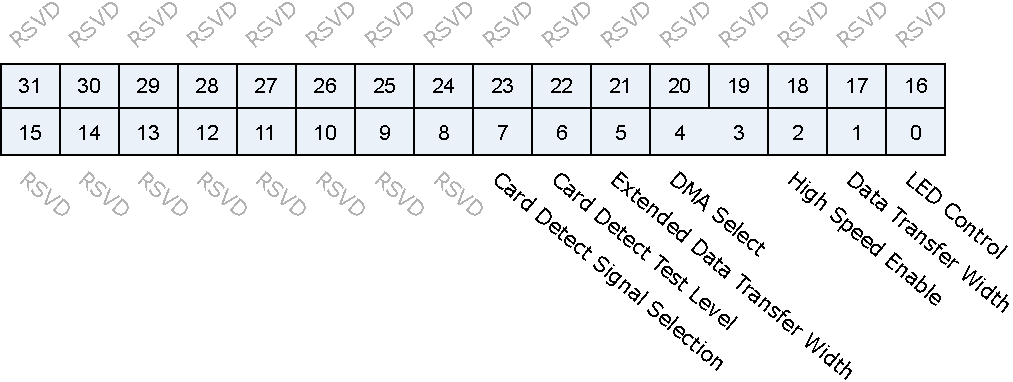
\includegraphics{SDH_Host_Control_1.pdf}
\end{figure}

\regdes{31:8&RSVD& & & \\\hline
7&CardDetect&r/w&1'b0&This bit selects source for the card detection.  \par   \par 1: The Card Detect Test Level is selected (for test purpose)  \par 0: SDCD\# is selected (for normal use)  \par   \par When the source for the card detection is switched, the interrupt should be disabled  \par during the switching period by clearing the Interrupt Status/Signal Enable register  \par in order to mask unexpected interrupt being caused by the glitch.  \par The Interrupt Status/Signal Enable should be disabled during over the period of  \par debouncing. 
\\\hline
6&CardDetect&r/w&1'b0&This bit is enabled while the Card Detect Signal Selection is set to 1 and it indicates  \par card inserted or not.  \par 1 Card Inserted  \par 0 No Card
\\\hline
5&ExtendedData&r/w&1'b0&This bit controls 8-bit bus width mode for embedded device. Support of this function  \par is indicated in 8-bit Support for Embedded Device in the Capabilities register. If a  \par device supports 8-bit bus mode, this bit may be set to 1. If this bit is 0, bus width is  \par controlled by Data Transfer Width in the Host Control 1 register.  \par This bit is not effective when multiple devices are installed on a bus slot (Slot Type \par is set to 10b in the Capabilities register). In this case, each device bus width is  \par controlled by Bus Width Preset field in the Shared Bus Control register.  \par 1: 8-bit Bus Width  \par 0 :Bus Width is Selected by Data Transfer Width
\\\hline
4:3&DMASelect&r/w&2'd0&One of supported DMA modes can be selected. The host driver shall check support  \par of DMA modes by referring the Capabilities register. Use of selected DMA is  \par determined by DMA Enable of the Transfer Mode register.  \par 00 SDMA is selected  \par 01 Reserved (New assignment is not allowed)  \par 10 32-bit Address ADMA2 is selected  \par 11 Reserved (will be modified by Version 4.00)
\\\hline
2&HighSpeed&r/w&1'b0& \par This bit is optional. Before setting this bit, the Host Driver shall check the High  \par Speed Support in the Capabilities register. If this bit is set to 0 (default), the Host  \par Controller outputs CMD line and DAT lines at the falling edge of the SD Clock (up to  \par 25MHz). If this bit is set to 1, the Host Controller outputs CMD line and DAT lines at  \par the rising edge of the SD Clock (up to 50MHz).  \par If Preset Value Enable in the Host Control 2 register is set to 1, Host Driver needs  \par to reset SD Clock Enable before changing this field to avoid generating clock  \par glitches. After setting this field, the Host Driver sets SD Clock Enable again.  \par 1 :High Speed mode  \par 0 :Normal Speed mode  \par 
\\\hline
1&DataTransfer&r/w&1'b0&This bit selects the data width of the Host Controller. The Host Driver shall set it to  \par match the data width of the SD card.  \par 1: 4-bit mode \par 0 :1-bit mode
\\\hline
0&LEDControl&r/w&1'b0&This bit is used to caution the user not to remove the card while the SD card is  \par being accessed. If the software is going to issue multiple SD commands, this bit  \par can be set during all these transactions. It is not necessary to change for each  \par transaction.  \par 1 :LED on  \par 0 :LED off 
\\\hline

}
\subsection{Power\_Control}
\label{SDH-Power-Control}
地址:0x20060029
 \begin{figure}[H]
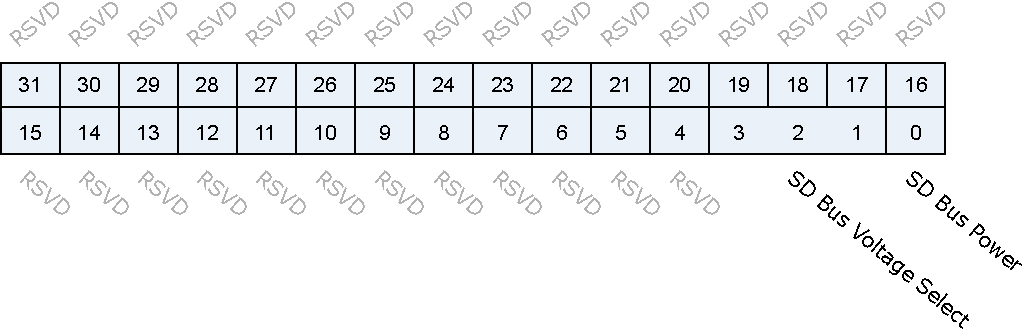
\includegraphics{SDH_Power_Control.pdf}
\end{figure}

\regdes{31:4&RSVD& & & \\\hline
3:1&SDBus&r/w&2'd0&SD Bus Voltage Select  \par By setting these bits, the Host Driver selects the voltage level for the SD card.  \par Before setting this register, the Host Driver shall check the Voltage Support bits in  \par the Capabilities register. If an unsupported voltage is selected, the Host System  \par shall not supply SD Bus voltage.  \par 111b 3.3V (Typ.)  \par 110b 3.0V (Typ.)  \par 101b 1.8V (Typ.)  \par 100b – 000b Reserved 
\\\hline
0&SDBus&r/w&1'b0&SD Bus Power  \par Before setting this bit, the SD Host Driver shall set SD Bus Voltage Select. If the  \par Host Controller detects the No Card state, this bit shall be cleared.  \par If this bit is cleared, the Host Controller shall immediately stop driving CMD and  \par DAT[3:0] (tri-state) and drive SDCLK to low level . 
\\\hline

}
\subsection{Block\_Gap\_Control}
\label{SDH-Block-Gap-Control}
地址:0x2006002a
 \begin{figure}[H]
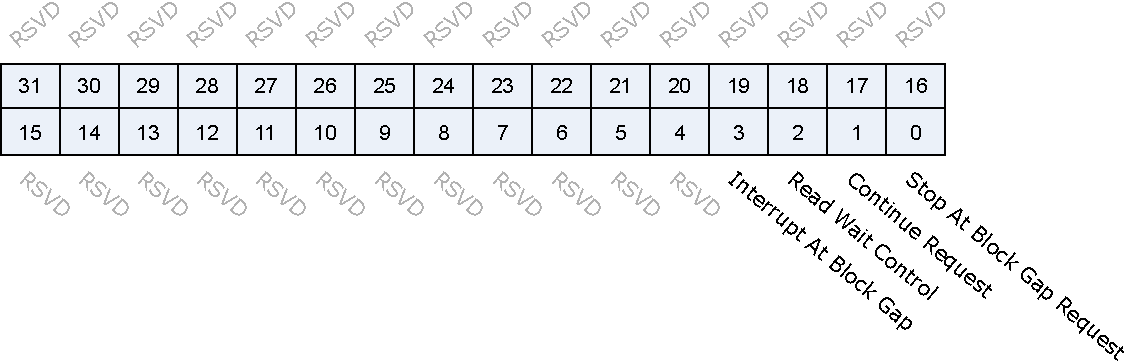
\includegraphics{SDH_Block_Gap_Control.pdf}
\end{figure}

\regdes{31:4&RSVD& & & \\\hline
3&InterruptAt&r/w&1'b0&Interrupt At Block Gap  \par This bit is valid only in 4-bit mode of the SDIO card and selects a sample point in  \par the interrupt cycle. Setting to 1 enables interrupt detection at the block gap for a  \par multiple block transfer. Setting to 0 disables interrupt detection during a multiple  \par block transfer. If the SD card cannot signal an interrupt during a multiple block  \par transfer, this bit should be set to 0. When the Host Driver detects an SD card  \par insertion, it shall set this bit according to the CCCR of the SDIO card. 
\\\hline
2&ReadWait&r/w&1'b0&Read Wait Control  \par The read wait function is optional for SDIO cards. If the card supports read wait,  \par set this bit to enable use of the read wait protocol to stop read data using the  \par DAT[2] line. Otherwise, the Host Controller has to stop the SD Clock to hold read  \par data, which restricts commands generation. When the Host Driver detects an SD  \par card insertion, it shall set this bit according to the CCCR of the SDIO card. If the  \par card does not support read wait, this bit shall never be set to 1 otherwise DAT line  \par conflict may occur. If this bit is set to 0, Suspend/Resume cannot be supported. 
\\\hline
1&ContinueRequest&r/w&1'b0&This bit is used to restart a transaction, which was stopped using the Stop At  \par Block Gap Request. To cancel stop at the block gap, set Stop At Block Gap  \par Request to 0 and set this bit 1 to restart the transfer.  \par The Host Controller automatically clears this bit in either of the following cases:  \par (1) In the case of a read transaction, the DAT Line Active changes from 0 to 1  \par as a read transaction restarts.  \par (2) In the case of a write transaction, the Write Transfer Active changes from 0  \par to 1 as the write transaction restarts.  \par Therefore, it is not necessary for Host Driver to set this bit to 0. If Stop At Block  \par Gap Request is set to 1, any write to this bit is ignored. 
\\\hline
0&StopAt&r/w&1'b0&This bit is used to stop executing read and write transaction at the next block gap  \par for non-DMA, SDMA and ADMA transfers. The Host Driver shall leave this bit set \par to 1 until the Transfer Complete is set to 1. Clearing both Stop At Block Gap  \par Request and Continue Request shall not cause the transaction to restart. When  \par Host Controller version is 1.00, the Host Driver can set this bit if the card supports  \par Read Wait Control. When Host Controller version is 2.00 or later, the Host Driver  \par can set this bit regardless of the card supports Read Wait Control. The Host  \par Controller shall stop read transfer by using Read Wait or stopping SD clock. In  \par case of write transfers in which the Host Driver writes data to the Buffer Data Port \par register, the Host Driver shall set this bit after all block data is written. If this bit is  \par set to 1, the Host Driver shall not write data to Buffer Data Port register.  \par This bit affects Read Transfer Active, Write Transfer Active, DAT Line Active \par and Command Inhibit (DAT) in the Present State register.  \par 
\\\hline

}
\subsection{Wakeup\_Control}
\label{SDH-Wakeup-Control}
地址:0x2006002b
 \begin{figure}[H]
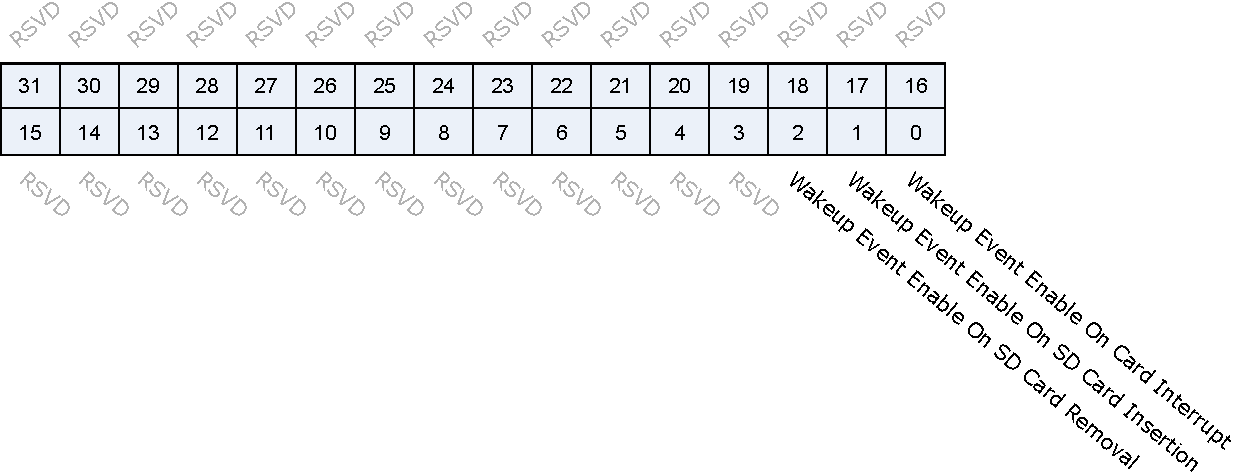
\includegraphics{SDH_Wakeup_Control.pdf}
\end{figure}

\regdes{31:3&RSVD& & & \\\hline
2&WakeupEvent&r/w&1'b0&Wakeup Event Enable On SD Card Removal  \par This bit enables wakeup event via Card Removal assertion in the Normal Interrupt  \par Status register. FN\_WUS (Wake Up Support) in CIS does not affect this bit. 
\\\hline
1&WakeupEvent&r/w&1'b0&Wakeup Event Enable On SD Card Insertion  \par This bit enables wakeup event via Card Insertion assertion in the Normal Interrupt  \par Status register. FN\_WUS (Wake Up Support) in CIS does not affect this bit. 
\\\hline
0&WakeupEvent&r/w&1'b0&Wakeup Event Enable On Card Interrupt  \par This bit enables wakeup event via Card Interrupt assertion in the Normal Interrupt  \par Status register. This bit can be set to 1 if FN\_WUS (Wake Up Support) in CIS is set  \par to 1.
\\\hline

}
\subsection{Clock\_Control}
\label{SDH-Clock-Control}
地址:0x2006002c
 \begin{figure}[H]
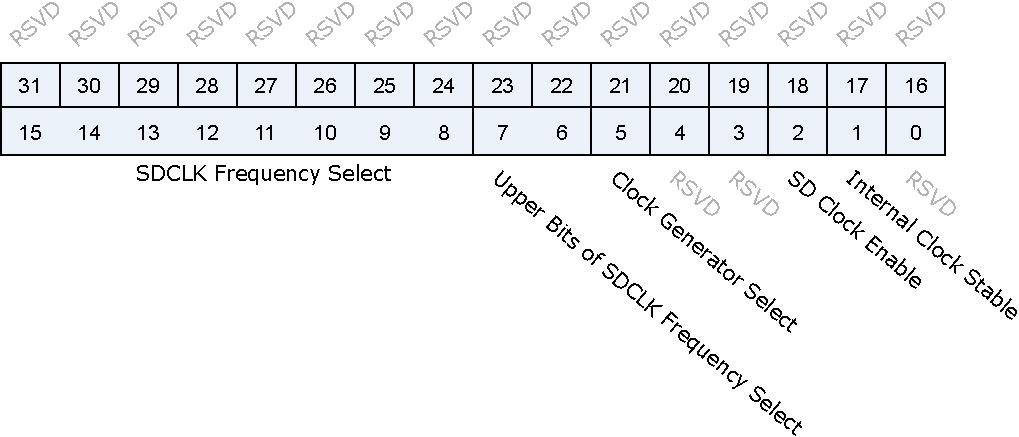
\includegraphics{SDH_Clock_Control.pdf}
\end{figure}

\regdes{31:16&RSVD& & & \\\hline
15:8&SDCLKFrequency&r/w&8'd0&SDCLK Frequency Select  \par This register is used to select the frequency of SDCLK pin. The definition of this  \par field is dependent on the Host Controller Version. 
\\\hline
7:6&UpperBits&roc/rw&2'd0&Upper Bits of SDCLK Frequency Select  \par Host Controller Version 1.00 and 2.00 do not support these bits and they are  \par treated as 00b fixed value (ROC).  \par Host Controller Version 3.00 shall support these bits to expand SDCLK  \par Frequency Select to 10-bit. Bit 07-06 is assigned to bit 09-08 of clock divider in  \par SDCLK Frequency Select. 
\\\hline
5&ClockGenerator&roc/rw&1'b0&Clock Generator Select  \par Host Controller Version 3.00 supports this bit. This bit is used to select the clock  \par generator mode in SDCLK Frequency Select. \par If the Programmable Clock Mode is supported (non-zero value is set to Clock  \par Multiplier in the Capabilities register), this bit attribute is RW, and if not  \par supported, this bit attribute is RO and zero is read.  \par This bit depends on the setting of Preset Value Enable in the Host Control 2 \par register.  \par If the Preset Value Enable = 0, this bit is set by Host Driver. \par If the Preset Value Enable = 1, this bit is automatically set to a value specified  \par in one of Preset Value registers. \par 1 Programmable Clock Mode  \par 0 Divided Clock Mode
\\\hline
4:3&RSVD& & & \\\hline
2&SDClock&rw&1'b0&SD Clock Enable  \par The Host Controller shall stop SDCLK when writing this bit to 0. SDCLK  \par Frequency Select can be changed when this bit is 0. Then, the Host Controller  \par shall maintain the same clock frequency until SDCLK is stopped (Stop at  \par SDCLK=0). If the Card Inserted in the Present State register is cleared, this bit  \par shall be cleared. 
\\\hline
1&InternalClock&roc&1'b0&Internal Clock Stable  \par This bit is set to 1 when SD Clock is stable after writing to Internal Clock  \par Enable in this register to 1. The SD Host Driver shall wait to set SD Clock  \par Enable until this bit is set to 1.  \par Note: This is useful when using PLL for a clock oscillator that requires setup  \par time. 
\\\hline
0&InternalClock&r/w&1'b0&Internal Clock Enable  \par This bit is set to 0 when the Host Driver is not using the Host Controller or the  \par Host Controller awaits a wakeup interrupt. The Host Controller should stop its  \par internal clock to go very low power state. Still, registers shall be able to be read  \par and written. Clock starts to oscillate when this bit is set to 1. When clock  \par oscillation is stable, the Host Controller shall set Internal Clock Stable in this  \par register to 1. This bit shall not affect card detection. 
\\\hline

}
\subsection{Timeout\_Control}
\label{SDH-Timeout-Control}
地址:0x2006002e
 \begin{figure}[H]
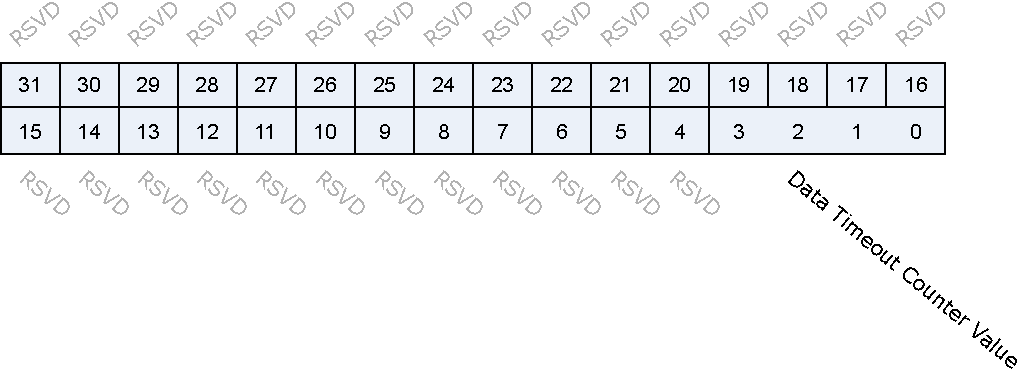
\includegraphics{SDH_Timeout_Control.pdf}
\end{figure}

\regdes{31:4&RSVD& & & \\\hline
3:0&DataTimeout&r/w&4'd0&Data Timeout Counter Value  \par This value determines the interval by which DAT line timeouts are detected. For  \par more information about timeout generation, refer to the Data Timeout Error in the  \par Error Interrupt Status register. Timeout clock frequency will be generated by  \par dividing the base clock TMCLK value by this value. When setting this register,  \par prevent inadvertent timeout events by clearing the Data Timeout Error Status  \par Enable (in the Error Interrupt Status Enable register)  \par 
\\\hline

}
\subsection{Software\_Reset}
\label{SDH-Software-Reset}
地址:0x2006002f
 \begin{figure}[H]
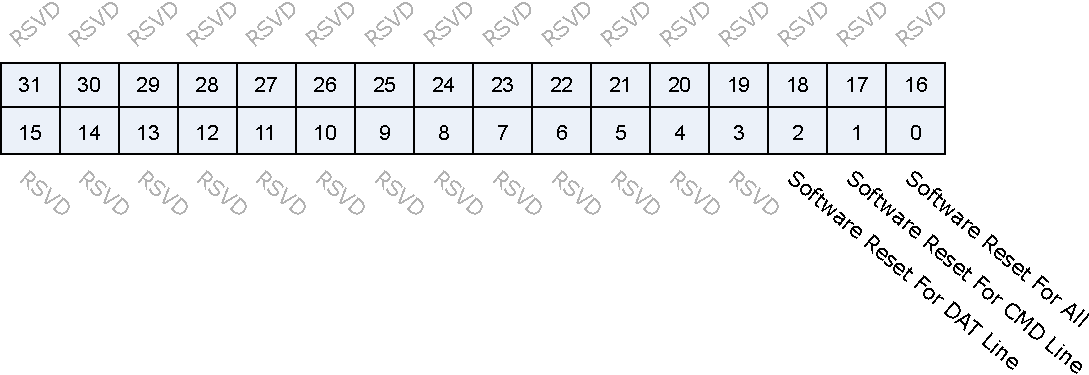
\includegraphics{SDH_Software_Reset.pdf}
\end{figure}

\regdes{31:3&RSVD& & & \\\hline
2&SoftwareReset&rwac&1'b0&Software Reset For DAT Line  \par Only part of data circuit is reset. DMA circuit is also reset. 
\\\hline
1&SoftwareReset&rwac&1'b0&Software Reset For CMD Line  \par Only part of command circuit is reset.  \par The following registers and bits are cleared by this bit:  \par Present State register \par Command Inhibit (CMD)  \par Normal Interrupt Status register \par Command Complete 
\\\hline
0&SoftwareReset&rwac&1'b0&Software Reset For All  \par This reset affects the entire Host Controller except for the card detection circuit.  \par Register bits of type ROC, RW, RW1C, RWAC are cleared to 0. During its  \par initialization, the Host Driver shall set this bit to 1 to reset the Host Controller. The  \par Host Controller shall reset this bit to 0 when Capabilities registers are valid and  \par the Host Driver can read them. Additional use of Software Reset For All may not  \par affect the value of the Capabilities registers. If this bit is set to 1, the host driver  \par should issue reset command and reinitialize the SD card. 
\\\hline

}
\subsection{Normal\_Interrupt\_Status}
\label{SDH-Normal-Interrupt-Status}
地址:0x20060030
 \begin{figure}[H]
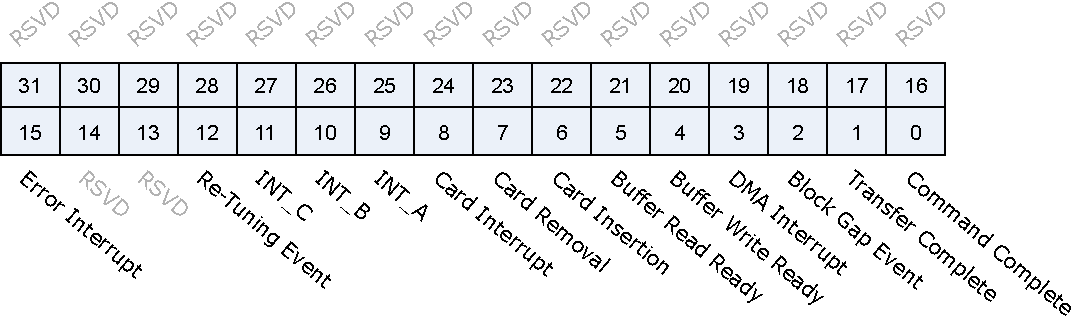
\includegraphics{SDH_Normal_Interrupt_Status.pdf}
\end{figure}

\regdes{31:16&RSVD& & & \\\hline
15&ErrorInterrupt&roc&1'b0&Error Interrupt  \par If any of the bits in the Error Interrupt Status register are set, then this bit is  \par set. Therefore the Host Driver can efficiently test for an error by checking  \par this bit first. This bit is read only. 
\\\hline
14:13&RSVD& & & \\\hline
12&Re-TuningEvent&roc&1'b0&Re-Tuning Event  \par This status is set if Re-Tuning Request in the Present State register  \par changes from 0 to 1.  \par Host Controller requests Host Driver to perform re-tuning for next data  \par transfer. Current data transfer (not large block count) can be completed  \par without re-tuning.
\\\hline
11&INT\_C&roc&1'b0&INT\_C  \par This status is set if INT\_C is enabled and INT\_C\# pin is in low level. Writing  \par this bit to 1 does not clear this bit. It is cleared by resetting the INT\_C  \par interrupt factor. Refer to the Shared Bus Control register.
\\\hline
10&INT\_B&roc&1'b0&INT\_B  \par This status is set if INT\_B is enabled and INT\_B\# pin is in low level. Writing  \par this bit to 1 does not clear this bit. It is cleared by resetting the INT\_B  \par interrupt factor. Refer to the Shared Bus Control register.
\\\hline
9&INT\_A&roc&1'b0&INT\_A  \par This status is set if INT\_A is enabled and INT\_A\# pin is in low level. Writing  \par this bit to 1 does not clear this bit. It is cleared by resetting the INT\_A  \par interrupt factor. Refer to the Shared Bus Control register. 
\\\hline
8&CardInterrupt&roc&1'b0&Card Interrupt  \par Writing this bit to 1 does not clear this bit. It is cleared by resetting the SD  \par card interrupt factor. In 1-bit mode, the Host Controller shall detect the Card  \par Interrupt without SD Clock to support wakeup. In 4-bit mode, the card  \par interrupt signal is sampled during the interrupt cycle, so there are some  \par sample delays between the interrupt signal from the SD card and the  \par interrupt to the Host System.  \par When this status has been set and the Host Driver needs to start this  \par interrupt service, Card Interrupt Status Enable in the Normal Interrupt  \par Status Enable register may be set to 0 in order to clear the card interrupt  \par statuses latched in the Host Controller and to stop driving the interrupt  \par signal to the Host System. After completion of the card interrupt service (It  \par should reset interrupt factors in the SD card and the interrupt signal may  \par not be asserted), set Card Interrupt Status Enable to 1 and start sampling  \par the interrupt signal again. \par Interrupt detected by DAT[1] is supported when there is a card per slot. In  \par case of shared bus, interrupt pins are used to detect interrupts. If 000b is  \par set to Interrupt Pin Select in the Shared Bus Control register, this status is  \par effective. Non-zero value is set to Interrupt Pin Select, INT\_A, INT\_B or  \par INT\_C is then used to device interrupts. 
\\\hline
7&CardRemoval&rw1c&1'b0&Card Removal  \par This status is set if the Card Inserted in the Present State register changes  \par from 1 to 0.  \par When the Host Driver writes this bit to 1 to clear this status, the status of the  \par Card Inserted in the Present State register should be confirmed. Because  \par the card detect state may possibly be changed when the Host Driver clear  \par this bit and interrupt event may not be generated. 
\\\hline
6&CardInsertion&rw1c&1'b0&Card Insertion  \par This status is set if the Card Inserted in the Present State register changes  \par from 0 to 1.  \par When the Host Driver writes this bit to 1 to clear this status, the status of the  \par Card Inserted in the Present State register should be confirmed. Because  \par the card detect state may possibly be changed when the Host Driver clear  \par this bit and interrupt event may not be generated. 
\\\hline
5&BufferRead&rw1c&1'b0&Buffer Read Ready  \par This status is set if the Buffer Read Enable changes from 0 to 1. Refer to  \par the Buffer Read Enable in the Present State register.  \par While performing tuning procedure (Execute Tuning is set to 1), Buffer  \par Read Ready is set to 1 for every CMD19 execution. 
\\\hline
4&BufferWrite&rw1c&1'b0&Buffer Write Ready  \par This status is set if the Buffer Write Enable changes from 0 to 1. Refer to  \par the Buffer Write Enable in the Present State register. 
\\\hline
3&DMAInterrupt&rw1c&1'b0&DMA Interrupt  \par This status is set if the Host Controller detects the Host SDMA Buffer \par boundary during transfer. Refer to the Host SDMA Buffer Boundary in the  \par Block Size register.  \par Other DMA interrupt factors may be added in the future.  \par In case of ADMA, by setting Int field in the descriptor table, Host Controller  \par generates this interrupt. Suppose that it is used for debugging.  \par This interrupt shall not be generated after the Transfer Complete. 
\\\hline
2&BlockGap&rw1c&1'b0&Block Gap Event  \par If the Stop At Block Gap Request in the Block Gap Control register is set,  \par this bit is set when both a read / write transaction is stopped at a block gap.  \par If Stop At Block Gap Request is not set to 1, this bit is not set to 1.  \par (1) In the case of a Read Transaction  \par This bit is set at the falling edge of the DAT Line Active Status (When  \par the transaction is stopped at SD Bus timing. The Read Wait shall be  \par supported in order to use this function. Refer to Section 3.12.3 about  \par the detail timing.  \par (2) Case of Write Transaction  \par This bit is set at the falling edge of Write Transfer Active Status (After  \par getting CRC status at SD Bus timing). Refer to Section 3.12.4 for more  \par details on the sequence of events. 
\\\hline
1&TransferComplete&rw1c&1'b0&Transfer Complete  \par This bit is set when a read / write transfer and a command with busy is  \par completed.  \par (1) In the case of a Read Transaction  \par This bit is set at the falling edge of Read Transfer Active Status.  \par This interrupt is generated in two cases. The first is when a data  \par transfer is completed as specified by data length (After the last data  \par has been read to the Host System). The second is when data has  \par stopped at the block gap and completed the data transfer by setting \par the Stop At Block Gap Request in the Block Gap Control register  \par (After valid data has been read to the Host System).  \par (2) In the case of a Write Transaction  \par This bit is set at the falling edge of the DAT Line Active Status. This  \par interrupt is generated in two cases. The first is when the last data is  \par written to the SD card as specified by data length and the busy signal  \par released. The second is when data transfers are stopped at the block  \par gap by setting Stop At Block Gap Request in the Block Gap Control \par register and data transfers completed. (After valid data is written to  \par the SD card and the busy signal released).  \par (3) In the case of a command with busy  \par This bit is set when busy is de-asserted. Refer to DAT Line Active \par and Command Inhibit (DAT) in the Present State register. 
\\\hline
0&CommandComplete&rw1c&1'b0&Command Complete  \par This bit is set when get the end bit of the command response. Auto CMD12  \par and Auto CMD23 consist of two responses. Command Complete is not  \par generated by the response of CMD12 or CMD23 but generated by the  \par response of a read/write command.  \par Refer to Command Inhibit (CMD) in the Present State register for how to  \par control this bit.  \par The table below shows that Command Timeout Error has higher priority  \par than Command Complete. If both bits are set to 1, it can be considered  \par that the response was not received correctly. 
\\\hline

}
\subsection{Error\_Interrupt\_Status}
\label{SDH-Error-Interrupt-Status}
地址:0x20060032
 \begin{figure}[H]
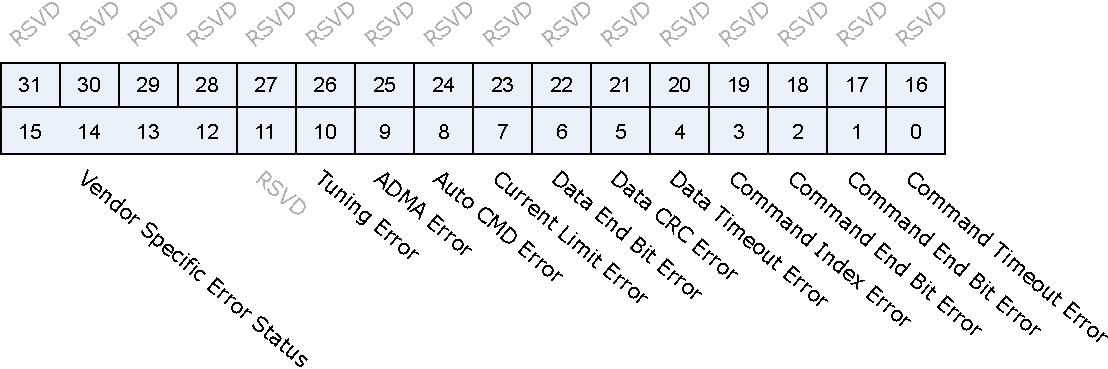
\includegraphics{SDH_Error_Interrupt_Status.pdf}
\end{figure}

\regdes{31:16&RSVD& & & \\\hline
15:12&VendorSpecific&rw1c&4'd0&Vendor Specific Error Status  \par Additional status bits can be defined in this register by the vendor. 
\\\hline
11&RSVD& & & \\\hline
10&TuningError&rw1c&1'b0&Tuning Error  \par This bit is set when an unrecoverable error is detected in a tuning circuit  \par except during tuning procedure (Occurrence of an error during tuning  \par procedure is indicated by Sampling Select). By detecting Tuning Error, Host  \par Driver needs to abort a command executing and perform tuning. To reset  \par tuning circuit, Sampling Clock shall be set to 0 before executing tuning  \par procedure . The Tuning Error is higher priority than the  \par other error interrupts generated during data transfer. By detecting Tuning  \par Error, the Host Driver should discard data transferred by a current read/write  \par command and retry data transfer after the Host Controller retrieved from  \par tuning circuit error.
\\\hline
9&ADMAError&rw1c&1'b0&ADMA Error  \par This bit is set when the Host Controller detects errors during ADMA based data  \par transfer. The state of the ADMA at an error occurrence is saved in the ADMA  \par Error Status Register,  \par In addition, the Host Controller generates this Interrupt when it detects invalid  \par descriptor data (Valid=0) at the ST\_FDS state. ADMA Error State in the \par ADMA Error Status indicates that an error occurs in ST\_FDS state. The Host  \par Driver may find that Valid bit is not set at the error descriptor.
\\\hline
8&AutoCMD&rw1c&1'b0&Auto CMD Error  \par Auto CMD12 and Auto CMD23 use this error status. This bit is set when  \par detecting that one of the bits D00-D04 in Auto CMD Error Status register has  \par changed from 0 to 1. In case of Auto CMD12, this bit is set to 1, not only when  \par the errors in Auto CMD12 occur but also when Auto CMD12 is not executed  \par due to the previous command error. 
\\\hline
7&CurrentLimit&rw1c&1'b0&Current Limit Error  \par By setting the SD Bus Power bit in the Power Control register, the Host  \par Controller is requested to supply power for the SD Bus. If the Host Controller  \par supports the Current Limit function, it can be protected from an illegal card by  \par stopping power supply to the card in which case this bit indicates a failure  \par status. Reading 1 means the Host Controller is not supplying power to SD card  \par due to some failure. Reading 0 means that the Host Controller is supplying  \par power and no error has occurred. The Host Controller may require some  \par sampling time to detect the current limit. If the Host Controller does not support  \par this function, this bit shall always be set to 0. 
\\\hline
6&DataEnd&rw1c&1'b0&Data End Bit Error  \par Occurs either when detecting 0 at the end bit position of read data which uses  \par the DAT line or at the end bit position of the CRC Status. 
\\\hline
5&DataCRC&rw1c&1'b0&Data CRC Error  \par Occurs when detecting CRC error when transferring read data which uses the  \par DAT line or when detecting the Write CRC status having a value of other than  \par "010". 
\\\hline
4&DataTimeout&rw1c&1'b0&Data Timeout Error  \par This bit is set when detecting one of following timeout conditions.  \par (1) Busy timeout for R1b,R5b type  \par (2) Busy timeout after Write CRC status  \par (3) Write CRC Status timeout  \par (4) Read Data timeout. 
\\\hline
3&CommandIndex&rw1c&1'b0&Command Index Error  \par This bit is set if a Command Index error occurs in the command response. 
\\\hline
2&CommandEnd&rw1c&1'b0&Command End Bit Error  \par This bit is set when detecting that the end bit of a command response is 0. 
\\\hline
1&CommandEnd&rw1c&1'b0&Command CRC Error  \par Command CRC Error is generated in two cases.  \par If a response is returned and the Command Timeout Error is set to 0  \par (indicating no timeout), this bit is set to 1 when detecting a CRC error in the  \par command response.  \par The Host Controller detects a CMD line conflict by monitoring the CMD line  \par when a command is issued. If the Host Controller drives the CMD line to 1  \par level, but detects 0 level on the CMD line at the next SD clock edge, then the  \par Host Controller shall abort the command (Stop driving CMD line) and set this  \par bit to 1. The Command Timeout Error shall also be set to 1 to distinguish CMD \par line conflict .
\\\hline
0&CommandTimeout&rw1c&1'b0&Command Timeout Error  \par This bit is set only if no response is returned within 64 SD clock cycles from the  \par end bit of the command. 
\\\hline

}
\subsection{Normal\_Interrupt\_Status\_Enable}
\label{SDH-Normal-Interrupt-Status-Enable}
地址:0x20060034
 \begin{figure}[H]
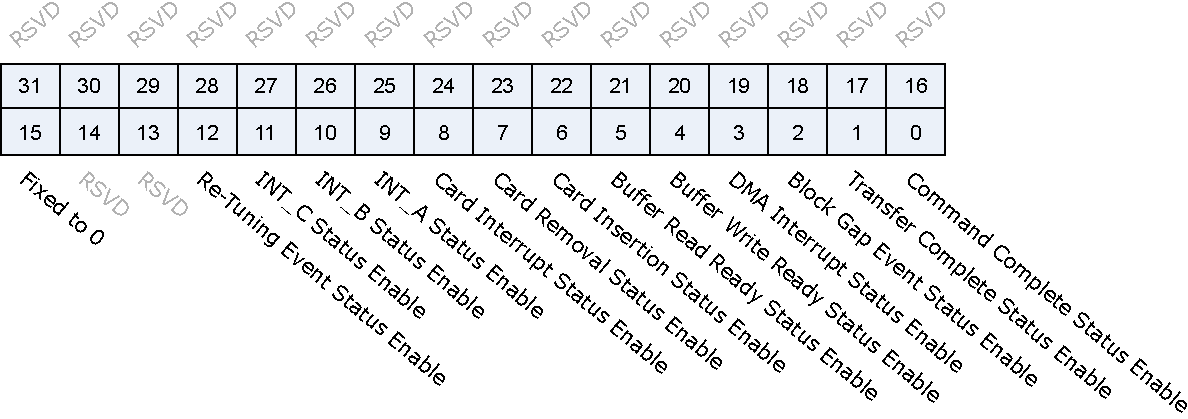
\includegraphics{SDH_Normal_Interrupt_Status_Enable.pdf}
\end{figure}

\regdes{31:16&RSVD& & & \\\hline
15&Fixedto&r&1'b0&Fixed to 0  \par The Host Driver shall control error interrupts using the Error Interrupt Status  \par Enable register. 
\\\hline
14:13&RSVD& & & \\\hline
12&Re-TuningEvent&r/w&1'b0&Re-Tuning Event Status Enable  \par 1 Enabled \par 0 Masked
\\\hline
11&INT\_CStatus&r/w&1'b0&INT\_C Status Enable  \par If this bit is set to 0, the Host Controller shall clear the interrupt request to the  \par System. The Host Driver may clear this bit before servicing the INT\_C and  \par may set this bit again after all interrupt requests to INT\_C pin are cleared to  \par prevent inadvertent interrupts. 
\\\hline
10&INT\_BStatus&r/w&1'b0&INT\_B Status Enable  \par If this bit is set to 0, the Host Controller shall clear the interrupt request to the  \par System. The Host Driver may clear this bit before servicing the INT\_B and  \par may set this bit again after all interrupt requests to INT\_B pin are cleared to  \par prevent inadvertent interrupts.
\\\hline
9&INT\_AStatus&r/w&1'b0&INT\_A Status Enable  \par If this bit is set to 0, the Host Controller shall clear the interrupt request to the  \par System. The Host Driver may clear this bit before servicing the INT\_A and  \par may set this bit again after all interrupt requests to INT\_A pin are cleared to  \par prevent inadvertent interrupts.
\\\hline
8&CardInterrupt&r/w&1'b0&If this bit is set to 0, the Host Controller shall clear interrupt request to the  \par System. The Card Interrupt detection is stopped when this bit is cleared  \par and restarted when this bit is set to 1. The Host Driver may clear the Card  \par Interrupt Status Enable before servicing the Card Interrupt and may set  \par this bit again after all interrupt requests from the card are cleared to prevent  \par inadvertent interrupts.
\\\hline
7&CardRemoval&r/w&1'b0&Card Removal Status Enable\\\hline
6&CardInsertion&r/w&1'b0&Card Insertion Status Enable\\\hline
5&BufferRead&r/w&1'b0&Buffer Read Ready Status Enable\\\hline
4&BufferWrite&r/w&1'b0&Buffer Write Ready Status Enable\\\hline
3&DMAInterrupt&r/w&1'b0&DMA Interrupt Status Enable\\\hline
2&BlockGap&r/w&1'b0&Block Gap Event Status Enable \\\hline
1&TransferComplete&r/w&1'b0&Transfer Complete Status Enable\\\hline
0&CommandComplete&r/w&1'b0&Command Complete Status Enable \\\hline

}
\subsection{Error\_Interrupt\_Status\_Enable}
\label{SDH-Error-Interrupt-Status-Enable}
地址:0x20060036
 \begin{figure}[H]
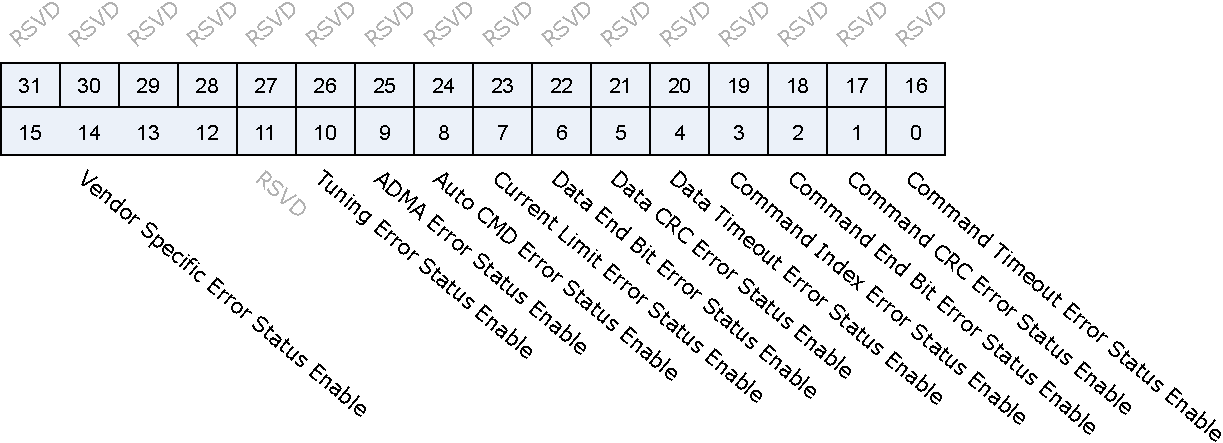
\includegraphics{SDH_Error_Interrupt_Status_Enable.pdf}
\end{figure}

\regdes{31:16&RSVD& & & \\\hline
15:12&VendorSpecific&r/w&4'd0&Vendor Specific Error Status Enable \\\hline
11&RSVD& & & \\\hline
10&TuningError&r/w&1'b0&Tuning Error Status Enable \\\hline
9&ADMAError&r/w&1'b0&ADMA Error Status Enable\\\hline
8&AutoCMD&r/w&1'b0&Auto CMD Error Status Enable\\\hline
7&CurrentLimit&r/w&1'b0&Current Limit Error Status Enable\\\hline
6&DataEnd&r/w&1'b0&Data End Bit Error Status Enable\\\hline
5&DataCRC&r/w&1'b0&Data CRC Error Status Enable\\\hline
4&DataTimeout&r/w&1'b0&Data Timeout Error Status Enable\\\hline
3&CommandIndex&r/w&1'b0&Command Index Error Status Enable\\\hline
2&CommandEnd&r/w&1'b0&Command End Bit Error Status Enable\\\hline
1&CommandCRC&r/w&1'b0&Command CRC Error Status Enable\\\hline
0&CommandTimeout&r/w&1'b0&Command Timeout Error Status Enable\\\hline

}
\subsection{Normal\_Interrupt\_Signal\_Enable}
\label{SDH-Normal-Interrupt-Signal-Enable}
地址:0x20060038
 \begin{figure}[H]
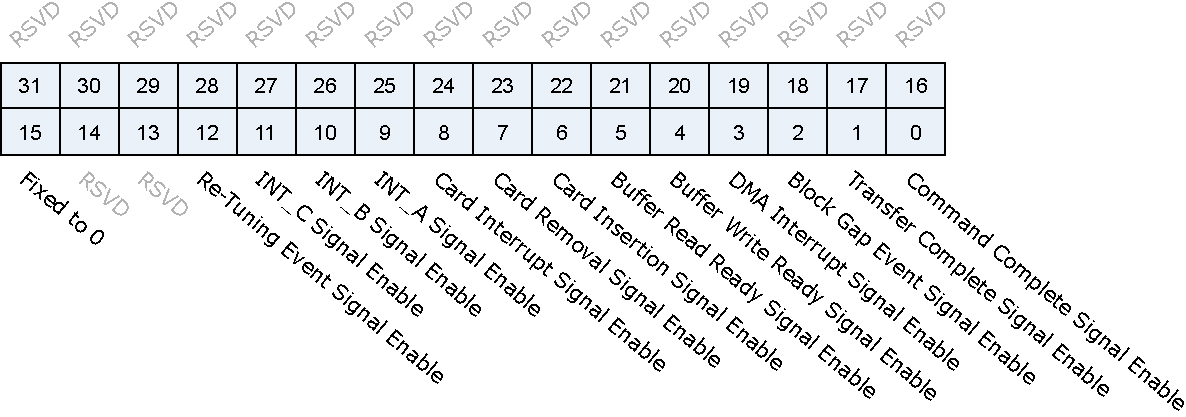
\includegraphics{SDH_Normal_Interrupt_Signal_Enable.pdf}
\end{figure}

\regdes{31:16&RSVD& & & \\\hline
15&Fixedto&r&1'b0&Fixed to 0  \par The Host Driver shall control error interrupts using the Error Interrupt Signal  \par Enable register.
\\\hline
14:13&RSVD& & & \\\hline
12&Re-TuningEvent&r/w&1'b0&Re-Tuning Event Signal Enable\\\hline
11&INT\_CSignal&r/w&1'b0&INT\_C Signal Enable\\\hline
10&INT\_BSignal&r/w&1'b0&INT\_B Signal Enable \\\hline
9&INT\_ASignal&r/w&1'b0&INT\_A Signal Enable\\\hline
8&CardInterrupt&r/w&1'b0&Card Interrupt Signal Enable\\\hline
7&CardRemoval&r/w&1'b0&Card Removal Signal Enable\\\hline
6&CardInsertion&r/w&1'b0&Card Insertion Signal Enable\\\hline
5&BufferRead&r/w&1'b0&Buffer Read Ready Signal Enable\\\hline
4&BufferWrite&r/w&1'b0&Buffer Write Ready Signal Enable \\\hline
3&DMAInterrupt&r/w&1'b0&DMA Interrupt Signal Enable\\\hline
2&BlockGap&r/w&1'b0&Block Gap Event Signal Enable\\\hline
1&TransferComplete&r/w&1'b0&Transfer Complete Signal Enable \\\hline
0&CommandComplete&r/w&1'b0&Command Complete Signal Enable \\\hline

}
\subsection{Error\_Interrupt\_Signal\_Enable}
\label{SDH-Error-Interrupt-Signal-Enable}
地址:0x2006003a
 \begin{figure}[H]
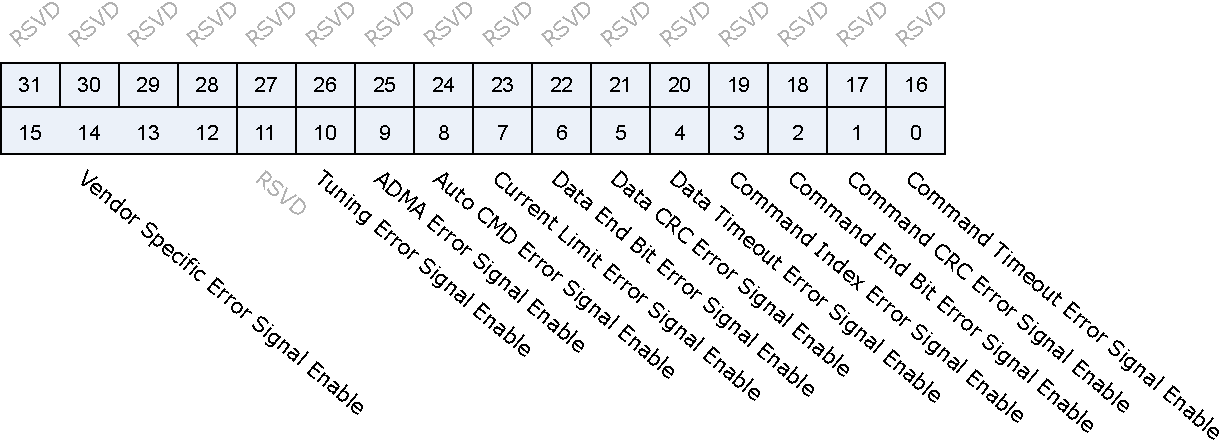
\includegraphics{SDH_Error_Interrupt_Signal_Enable.pdf}
\end{figure}

\regdes{31:16&RSVD& & & \\\hline
15:12&VendorSpecific&r/w&4'd0&Vendor Specific Error Signal Enable\\\hline
11&RSVD& & & \\\hline
10&TuningError&r/w&1'b0&Tuning Error Signal Enable\\\hline
9&ADMAError&r/w&1'b0&ADMA Error Signal Enable\\\hline
8&AutoCMD&r/w&1'b0&Auto CMD Error Signal Enable \\\hline
7&CurrentLimit&r/w&1'b0&Current Limit Error Signal Enable\\\hline
6&DataEnd&r/w&1'b0&Data End Bit Error Signal Enable\\\hline
5&DataCRC&r/w&1'b0&Data CRC Error Signal Enable\\\hline
4&DataTimeout&r/w&1'b0&Data Timeout Error Signal Enable \\\hline
3&CommandIndex&r/w&1'b0&Command Index Error Signal Enable \\\hline
2&CommandEnd&r/w&1'b0&Command End Bit Error Signal Enable\\\hline
1&CommandCRC&r/w&1'b0&Command CRC Error Signal Enable\\\hline
0&CommandTimeout&r/w&1'b0&Command Timeout Error Signal Enable\\\hline

}
\subsection{Auto\_CMD\_Error\_Status}
\label{SDH-Auto-CMD-Error-Status}
地址:0x2006003c
 \begin{figure}[H]
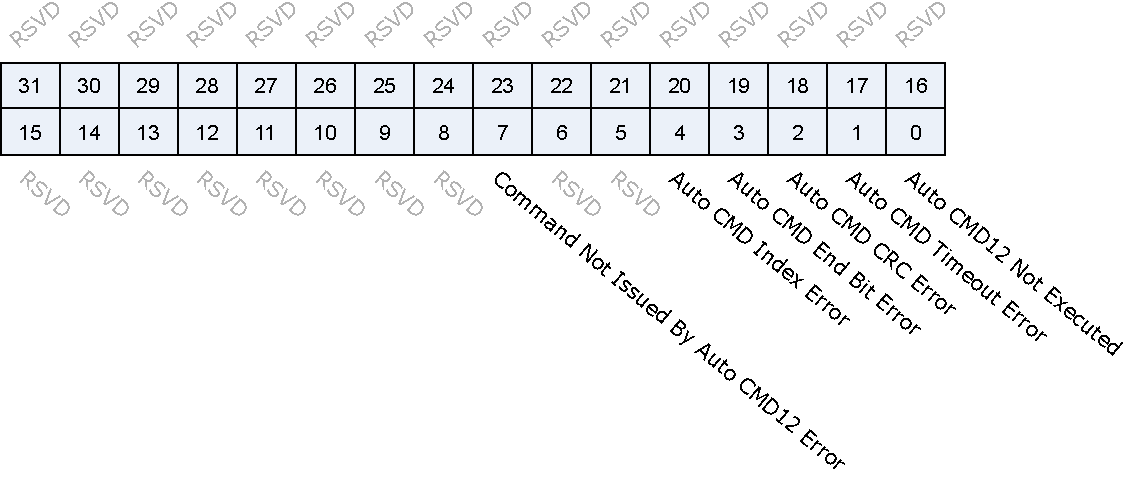
\includegraphics{SDH_Auto_CMD_Error_Status.pdf}
\end{figure}

\regdes{31:8&RSVD& & & \\\hline
7&CommandNot&roc&1'b0&Command Not Issued By Auto CMD12 Error  \par Setting this bit to 1 means CMD\_wo\_DAT is not executed due to an Auto  \par CMD12 Error (D04-D01) in this register.  \par This bit is set to 0 when Auto CMD Error is generated by Auto CMD23. 
\\\hline
6:5&RSVD& & & \\\hline
4&AutoCMD&roc&1'b0&Auto CMD Index Error  \par This bit is set if the Command Index error occurs in response to a command.
\\\hline
3&AutoCMD&roc&1'b0&Auto CMD End Bit Error  \par This bit is set when detecting that the end bit of command response is 0. 
\\\hline
2&AutoCMD&roc&1'b0&Auto CMD CRC Error\\\hline
1&AutoCMD&roc&1'b0&Auto CMD Timeout Error\\\hline
0&AutoCMD12&roc&1'b0&Auto CMD12 Not Executed\\\hline

}
\subsection{Host\_Control\_2}
\label{SDH-Host-Control-2}
地址:0x2006003e
 \begin{figure}[H]
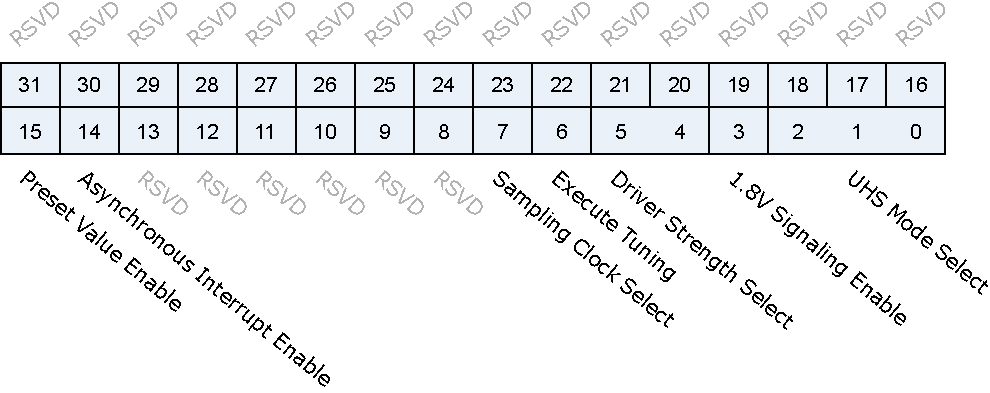
\includegraphics{SDH_Host_Control_2.pdf}
\end{figure}

\regdes{31:16&RSVD& & & \\\hline
15&PresetValue&r/w&1'b0&Preset Value Enable  \par Host Controller Version 3.00 supports this bit. \par As the operating SDCLK frequency and I/O driver strength depend on the  \par Host System implementation, it is difficult to determine these parameters in  \par the Standard Host Driver. When Preset Value Enable is set, automatic  \par SDCLK frequency generation and driver strength selection is performed  \par without considering system specific conditions. This bit enables the  \par functions defined in the Preset Value registers.
\\\hline
14&AsynchronousInterrupt&r/w&1'b0&Asynchronous Interrupt Enable  \par This bit can be set to 1 if a card supports asynchronous interrupts and  \par Asynchronous Interrupt Support is set to 1 in the Capabilities register.  \par Asynchronous interrupt is effective when DAT[1] interrupt is used in 4-bit SD  \par mode (and zero is set to Interrupt Pin Select in the Shared Bus Control \par register). If this bit is set to 1, the Host Driver can stop the SDCLK during  \par asynchronous interrupt period to save power. During this period, the Host  \par Controller continues to deliver the Card Interrupt to the host when it is  \par asserted by the Card.
\\\hline
13:8&RSVD& & & \\\hline
7&SamplingClock&r/w&1'b0&Sampling Clock Select  \par Host Controller uses this bit to select sampling clock to receive CMD and  \par DAT. This bit is set by tuning procedure and valid after the completion of  \par tuning (when Execute Tuning is cleared). Setting 1 means that tuning is  \par completed successfully and setting 0 means that tuning is failed. Writing 1 to  \par this bit is meaningless and ignored. A tuning circuit is reset by writing to 0.  \par This bit can be cleared with setting Execute Tuning. Once the tuning circuit  \par is reset, it will take time to complete tuning sequence. Therefore, Host Driver  \par should keep this bit to 1 to perform re-tuning sequence to compete re-tuning  \par sequence in a short time. Change of this bit is not allowed while the Host  \par Controller is receiving response or a read data block. 
\\\hline
6&ExecuteTuning&rwac&1'b0&Execute Tuning  \par This bit is set to 1 to start tuning procedure and automatically cleared when  \par tuning procedure is completed. The result of tuning is indicated to Sampling  \par Clock Select. Tuning procedure is aborted by writing 0. Refer to Figure 2-29  \par for more detail about tuning procedure.
\\\hline
5:4&DriverStrength&r/w&2'd0&Driver Strength Select  \par Host Controller output driver in 1.8V signaling is selected by this bit. In 3.3V  \par signaling, this field is not effective. This field can be set depends on Driver  \par Type A, C and D support bits in the Capabilities register.  \par This bit depends on setting of Preset Value Enable.  \par If Preset Value Enable = 0, this field is set by Host Driver. \par If Preset Value Enable = 1, this field is automatically set by a value  \par specified in the one of Preset Value registers.
\\\hline
3&1.8VSignaling&r/w&1'b0&1.8V Signaling Enable  \par This bit controls voltage regulator for I/O cell. 3.3V is supplied to the card  \par regardless of signaling voltage.  \par Setting this bit from 0 to 1 starts changing signal voltage from 3.3V to 1.8V.  \par 1.8V regulator output shall be stable within 5ms. Host Controller clears this  \par bit if switching to 1.8V signaling fails.  \par Clearing this bit from 1 to 0 starts changing signal voltage from 1.8V to 3.3V.  \par 3.3V regulator output shall be stable within 5ms.  \par Host Driver can set this bit to 1 when Host Controller supports 1.8V signaling  \par (One of support bits is set to 1: SDR50, SDR104 or DDR50 in the  \par Capabilities register) and the card or device supports UHS-I (S18A=1. Refer  \par to Bus Signal Voltage Switch Sequence in the Physical Layer Specification  \par Version 3.0x). 
\\\hline
2:0&UHSMode&r/w&3'd0&UHS Mode Select  \par This field is used to select one of UHS-I modes and effective when 1.8V  \par Signaling Enable is set to 1.
\\\hline

}
\subsection{Capabilities\_1}
\label{SDH-Capabilities-1}
地址:0x20060040
 \begin{figure}[H]
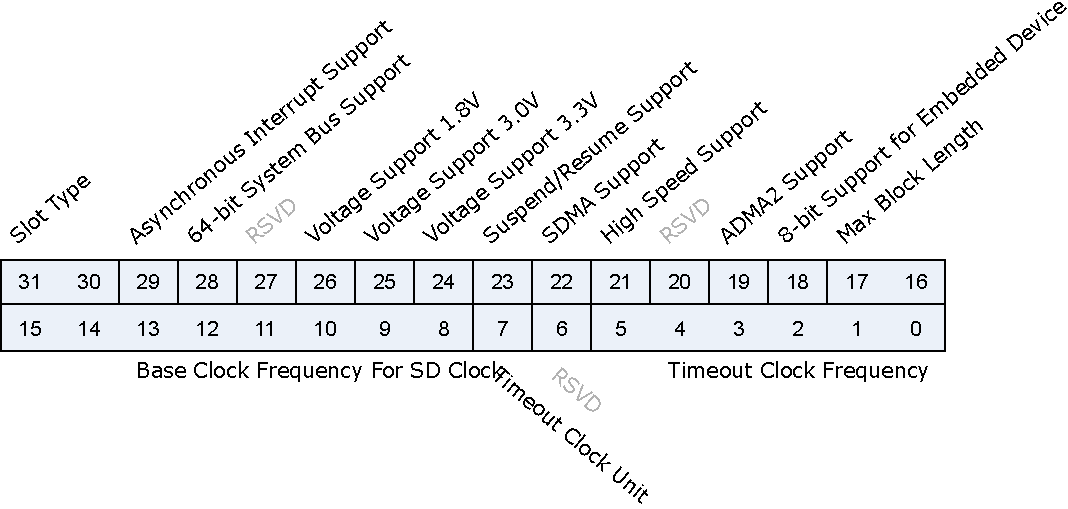
\includegraphics{SDH_Capabilities_1.pdf}
\end{figure}

\regdes{31:30&SlotType&HwInit&2'd0&Slot Type  \par This field indicates usage of a slot by a specific Host System. (A host  \par controller register set is defined per slot.) Embedded Slot for One Device  \par (01b) means that only one non-removable device is connected to a SD bus  \par slot. Shared Bus Slot (10b) can be set if Host Controller supports Shared  \par Bus Control register.  \par The Standard Host Driver controls only a removable card or one embedded  \par device connected to a SD bus slot. If a slot is configured for shared bus  \par (10b), the Standard Host Driver does not control embedded devices  \par connected to a shared bus. Shared bus slot is controlled by a specific host  \par driver developed by a Host System.  \par 00b Removable Card Slot  \par 01b Embedded Slot for One Device  \par 10b Shared Bus Slot  \par 11b Reserved
\\\hline
29&AsynchronousInterrupt&HwInit&1'b0&Asynchronous Interrupt Support  \par Refer to SDIO Specification Version 3.00 about asynchronous interrupt. 
\\\hline
28&64-bitSystem&HwInit&1'b0&64-bit System Bus Support  \par Setting 1 to this bit indicates that the Host Controller supports 64-bit  \par address descriptor mode and is connected to 64-bit address system bus.
\\\hline
27&RSVD& & & \\\hline
26&VoltageSupport&HwInit&1'b0&Voltage Support 1.8V  \par Embedded system can use 1.8V power supply. 
\\\hline
25&VoltageSupport&HwInit&1'b0&Voltage Support 3.0V  \par 1 :3.0V Supported  \par 0 :3.0V Not Supported
\\\hline
24&VoltageSupport&HwInit&1'b0&Voltage Support 3.3V\\\hline
23&Suspend/ResumeSupport&HwInit&1'b0&Suspend/Resume Support  \par This bit indicates whether the Host Controller supports Suspend / Resume  \par functionality. If this bit is 0, the Host Driver shall not issue either Suspend or  \par Resume commands because the Suspend and Resume mechanism is not supported. 
\\\hline
22&SDMASupport&HwInit&1'b0&SDMA Support  \par This bit indicates whether the Host Controller is capable of using SDMA to  \par transfer data between system memory and the Host Controller directly.
\\\hline
21&HighSpeed&HwInit&1'b0&High Speed Support  \par This bit indicates whether the Host Controller and the Host System support  \par High Speed mode and they can supply SD Clock frequency from 25MHz to  \par 50MHz. 
\\\hline
20&RSVD& & & \\\hline
19&ADMA2Support&HwInit&1'b0&ADMA2 Support  \par This bit indicates whether the Host Controller is capable of using ADMA2. 
\\\hline
18&8-bitSupport&HwInit&1'b0&8-bit Support for Embedded Device  \par This bit indicates whether the Host Controller is capable of using 8-bit bus  \par width mode. This bit is not effective when Slot Type is set to 10b. In this  \par case, refer to Bus Width Preset in the Shared Bus resister.
\\\hline
17:16&MaxBlock&HwInit&2'd0&Max Block Length  \par This value indicates the maximum block size that the Host Driver can read  \par and write to the buffer in the Host Controller. The buffer shall transfer this  \par block size without wait cycles. Three sizes can be defined as indicated  \par below. It is noted that transfer block length shall be always 512 bytes for SD  \par Memory Cards regardless this field.
\\\hline
15:8&BaseClock&HwInit&8'd0&Base Clock Frequency For SD Clock  \par This value indicates the base (maximum) clock frequency for the SD Clock.  \par Definition of this field depends on Host Controller Version.
\\\hline
7&TimeoutClock&HwInit&1'b0&Timeout Clock Unit  \par This bit shows the unit of base clock frequency used to detect Data Timeout  \par Error. 
\\\hline
6&RSVD& & & \\\hline
5:0&TimeoutClock&HwInit&6'd0&Timeout Clock Frequency \par This bit shows the base clock frequency used to detect Data Timeout Error. \par The Timeout Clock Unit defines the unit of this field's value. 
\\\hline

}
\subsection{Capabilities\_2}
\label{SDH-Capabilities-2}
地址:0x20060044
 \begin{figure}[H]
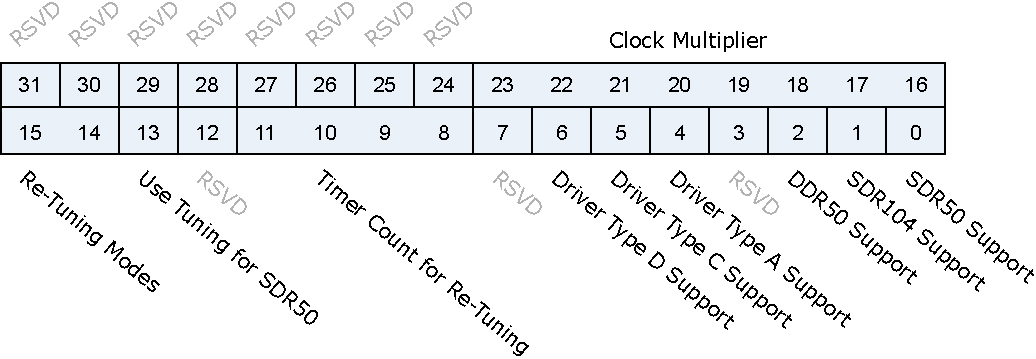
\includegraphics{SDH_Capabilities_2.pdf}
\end{figure}

\regdes{31:24&RSVD& & & \\\hline
23:16&ClockMultiplier&HwInit&8'd0&Clock Multiplier  \par This field indicates clock multiplier value of programmable clock generator.  \par Refer to Clock Control register. Setting 00h means that Host Controller  \par does not support programmable clock generator. 
\\\hline
15:14&Re-TuningModes&HwInit&2'd0&Re-Tuning Modes  \par This field selects re-tuning method and limits the maximum data length. 
\\\hline
13&UseTuning&HwInit&1'b0&Use Tuning for SDR50  \par If this bit is set to 1, this Host Controller requires tuning to operate SDR50. \par (Tuning is always required to operate SDR104.) 
\\\hline
12&RSVD& & & \\\hline
11:8&TimerCount&HwInit&4'd0&Timer Count for Re-Tuning  \par This field indicates an initial value of the Re-Tuning Timer for Re-Tuning  \par Mode 1 to 3. Setting to 0 disables Re-Tuning Timer. 
\\\hline
7&RSVD& & & \\\hline
6&DriverType&HwInit&1'b0&Driver Type D Support  \par This bit indicates support of Driver Type D for 1.8 Signaling. 
\\\hline
5&DriverType&HwInit&1'b0&Driver Type C Support  \par This bit indicates support of Driver Type C for 1.8 Signaling. 
\\\hline
4&DriverType&HwInit&1'b0&Driver Type A Support  \par This bit indicates support of Driver Type A for 1.8 Signaling.
\\\hline
3&RSVD& & & \\\hline
2&DDR50Support&HwInit&1'b0&DDR50 Support\\\hline
1&SDR104Support&HwInit&1'b0&SDR104 Support  \par SDR104 requires tuning.
\\\hline
0&SDR50Support&HwInit&1'b0&SDR50 Support  \par If SDR104 is supported, this bit shall be set to 1. Bit 45 indicates whether  \par SDR50 requires tuning or not. 
\\\hline

}
\subsection{Maximum\_Current\_Capabilities}
\label{SDH-Maximum-Current-Capabilities}
地址:0x20060048
 \begin{figure}[H]
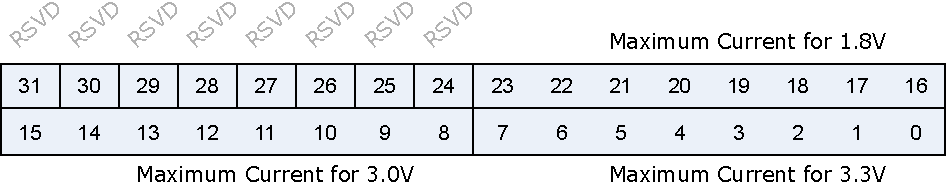
\includegraphics{SDH_Maximum_Current_Capabilities.pdf}
\end{figure}

\regdes{31:24&RSVD& & & \\\hline
23:16&MaximumCurrent&HwInit&8'd0&Maximum Current for 1.8V\\\hline
15:8&MaximumCurrent&HwInit&8'd0&Maximum Current for 3.0V\\\hline
7:0&MaximumCurrent&HwInit&8'd0&Maximum Current for 3.3V\\\hline

}
\subsection{Force\_Event\_Register\_for\_Auto\_CMD\_Error\_Status}
\label{SDH-Force-Event-Register-for-Auto-CMD-Error-Status}
地址:0x20060050
 \begin{figure}[H]
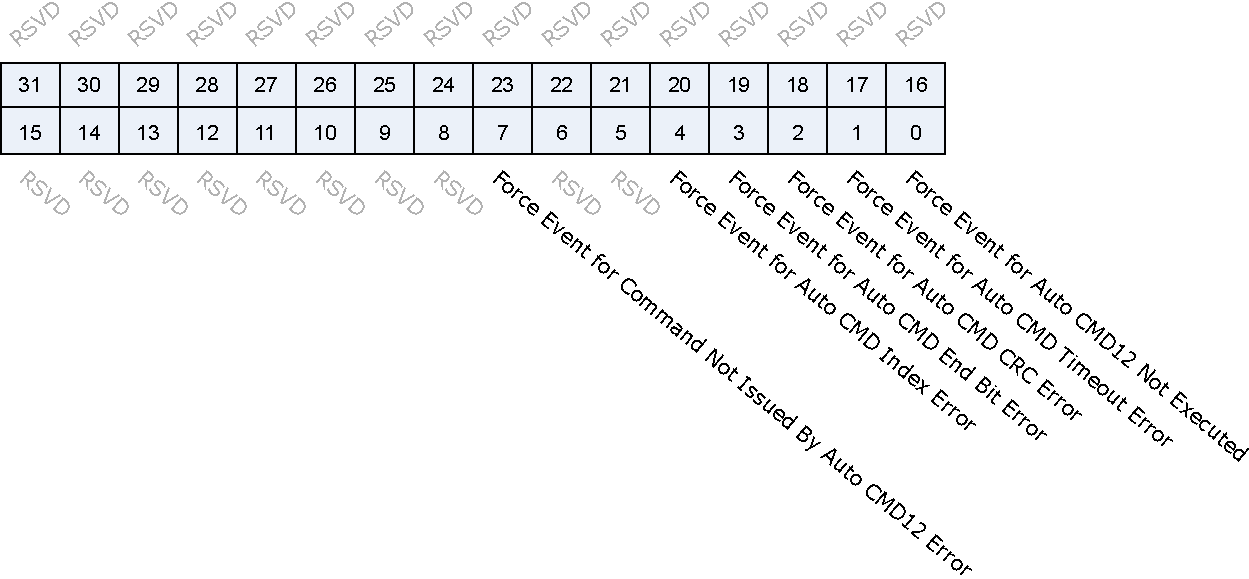
\includegraphics{SDH_Force_Event_Register_for_Auto_CMD_Error_Status.pdf}
\end{figure}

\regdes{31:8&RSVD& & & \\\hline
7&ForceEvent&w&x&Force Event for Command Not Issued By Auto CMD12 Error\\\hline
6:5&RSVD& & & \\\hline
4&ForceEvent&w&x&Force Event for Auto CMD Index Error \\\hline
3&ForceEvent&w&x&Force Event for Auto CMD End Bit Error\\\hline
2&ForceEvent&w&x&Force Event for Auto CMD CRC Error \\\hline
1&ForceEvent&w&x&Force Event for Auto CMD Timeout Error \\\hline
0&ForceEvent&w&x&Force Event for Auto CMD12 Not Executed\\\hline

}
\subsection{Force\_Event\_Register\_for\_Error\_Interrupt\_Status}
\label{SDH-Force-Event-Register-for-Error-Interrupt-Status}
地址:0x20060052
 \begin{figure}[H]
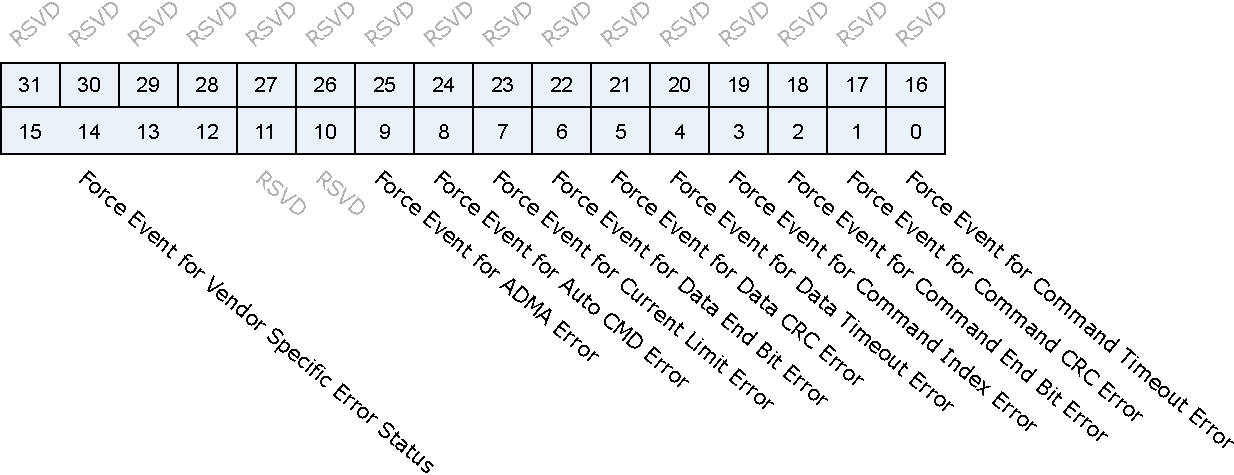
\includegraphics{SDH_Force_Event_Register_for_Error_Interrupt_Status.pdf}
\end{figure}

\regdes{31:16&RSVD& & & \\\hline
15:12&ForceEvent&w&x&Force Event for Vendor Specific Error Status  \par Additional status bits can be defined in this register by the vendor.
\\\hline
11:10&RSVD& & & \\\hline
9&ForceEvent&w&x&Force Event for ADMA Error\\\hline
8&ForceEvent&w&x&Force Event for Auto CMD Error\\\hline
7&ForceEvent&w&x&Force Event for Current Limit Error \\\hline
6&ForceEvent&w&x&Force Event for Data End Bit Error\\\hline
5&ForceEvent&w&x&Force Event for Data CRC Error\\\hline
4&ForceEvent&w&x&Force Event for Data Timeout Error\\\hline
3&ForceEvent&w&x&Force Event for Command Index Error\\\hline
2&ForceEvent&w&x&Force Event for Command End Bit Error\\\hline
1&ForceEvent&w&x&Force Event for Command CRC Error\\\hline
0&ForceEvent&w&x&Force Event for Command Timeout Error \\\hline

}
\subsection{ADMA\_Error\_Status}
\label{SDH-ADMA-Error-Status}
地址:0x20060054
 \begin{figure}[H]
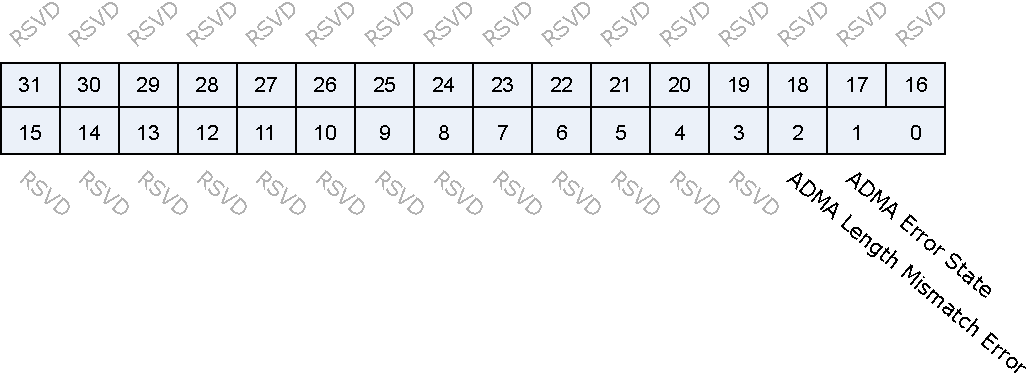
\includegraphics{SDH_ADMA_Error_Status.pdf}
\end{figure}

\regdes{31:3&RSVD& & & \\\hline
2&ADMALength&roc&1'b0&ADMA Length Mismatch Error  \par This error occurs in the following 2 cases.  \par (1) While Block Count Enable being set, the total data length specified by the  \par Descriptor table is different from that specified by the Block Count and  \par Block Length.  \par (2) Total data length can not be divided by the block length. 
\\\hline
1:0&ADMAError&roc&1'b0&ADMA Error State  \par This field indicates the state of ADMA when error is occurred during ADMA data  \par transfer. This field never indicates "10" because ADMA never stops in this state.
\\\hline

}
\subsection{Shared\_Bus\_Control}
\label{SDH-Shared-Bus-Control}
地址:0x200600e0
 \begin{figure}[H]
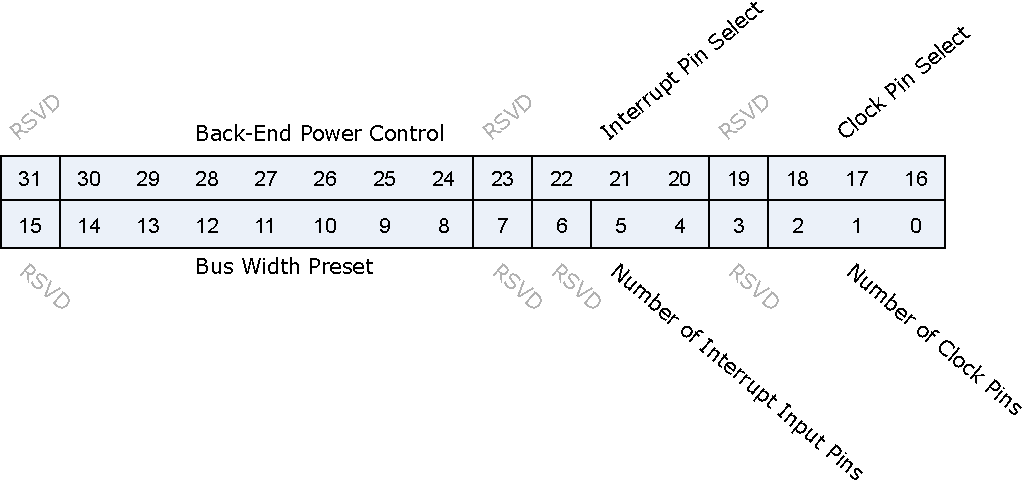
\includegraphics{SDH_Shared_Bus_Control.pdf}
\end{figure}

\regdes{31&RSVD& & & \\\hline
30:24&Back-EndPower&r/w&7'd0&Back-End Power Control  \par Each bit of this field controls back-end power supply for an embedded  \par device. Host interface voltage (VDDH) is not controlled by this field. The  \par number of devices supported is specified by Number of Clock Pins and a  \par maximum of 7 devices can be controlled. 
\\\hline
23&RSVD& & & \\\hline
22:20&InterruptPin&r/w&3'd0&Interrupt Pin Select  \par Interrupt pin inputs are enabled by this field. Enable of unsupported  \par interrupt pin is meaningless. 
\\\hline
19&RSVD& & & \\\hline
18:16&ClockPin&r/w&3'd0&Clock Pin Select  \par One of clock pin outputs is selected by this field. Select of unsupported  \par clock pin is meaningless. Refer to Figure 2-38 for the timing of clock  \par outputs.
\\\hline
15&RSVD& & & \\\hline
14:8&BusWidth&r/w&7'd0&Bus Width Preset  \par Shared bus supports mixing of 4-bit and 8-bit bus width devices.  \par Each bit of this field specifies the bus width for each embedded device. The  \par number of devices supported is specified by Number of Clock Pins and a  \par maximum of 7 devices are supported.  \par This field is effective when multiple devices are connected to a shared bus  \par (Slot Type is set to 10b in the Capabilities register). In the other case,  \par Extended Data Transfer Width in the Host Control 1 register is used to  \par select 8-bit bus width. As use of 1-bit mode is not intended for shared bus,  \par Data Transfer Width in the Host Control 1 register should be set to 1. 
\\\hline
7:6&RSVD& & & \\\hline
5:4&Numberof&r/w&2'd0&Number of Interrupt Input Pins  \par This field indicates support of interrupt input pins for shared bus system.  \par Three asynchronous interrupt pins are defined, INT\_A\#, INT\_B\# and  \par INT\_C\#. Which interrupt pin is used is determined by the system. Each one  \par is driven by open drain and then wired or connection is possible. 
\\\hline
3&RSVD& & & \\\hline
2:0&Numberof&HwInit&3'd0&Number of Clock Pins  \par This field indicates support of clock pins to select one of devices for shared  \par bus system. Up to 7 clock pins can be supported.  \par Shared bus is supported by specific system. Then Standard Host Driver  \par does not support control of these clock pins. 
\\\hline

}
\subsection{Slot\_Interrupt\_Status}
\label{SDH-Slot-Interrupt-Status}
地址:0x200600fc
 \begin{figure}[H]
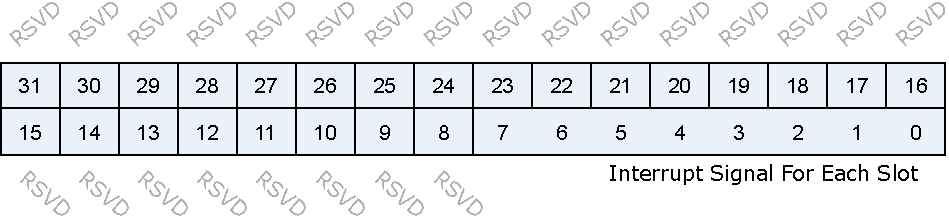
\includegraphics{SDH_Slot_Interrupt_Status.pdf}
\end{figure}

\regdes{31:8&RSVD& & & \\\hline
7:0&InterruptSignal&roc&8'd0&Interrupt Signal For Each Slot  \par These status bits indicate the logical OR of Interrupt Signal and Wakeup  \par Signal for each slot. A maximum of 8 slots can be defined. If one interrupt  \par signal is associated with multiple slots, the Host Driver can know which  \par interrupt is generated by reading these status bits. By a power on reset or by  \par setting Software Reset For All, the interrupt signal shall be de-asserted  \par and this status shall read 00h. 
\\\hline

}
\subsection{Host\_Controller\_Version}
\label{SDH-Host-Controller-Version}
地址:0x200600fe
 \begin{figure}[H]
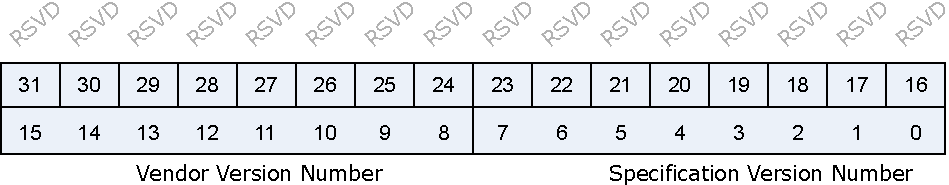
\includegraphics{SDH_Host_Controller_Version.pdf}
\end{figure}

\regdes{31:16&RSVD& & & \\\hline
15:8&VendorVersion&HwInit&8'd0&Vendor Version Number  \par This status is reserved for the vendor version number. The Host Driver  \par should not use this status.
\\\hline
7:0&SpecificationVersion&HwInit&8'd0&Specification Version Number  \par This status indicates the Host Controller Spec. Version. The upper and  \par lower 4-bits indicate the version.  \par  \par 00h SD Host Specification Version 1.00  \par 01h SD Host Specification Version 2.00  \par Including the feature of the ADMA and Test Register,  \par 02h SD Host Specification Version 3.00  \par others Reserved 
\\\hline

}
